% !TEX program = xelatex
\documentclass[a4paper,14pt,oneside,openany]{memoir}

%%% Задаем поля, отступы и межстрочный интервал %%%
\usepackage{amsmath}
\usepackage[left=30mm, right=15mm, top=20mm, bottom=20mm]{geometry} % Пакет geometry с аргументами для определения полей
\pagestyle{plain} % Убираем стандарные для данного класса верхние колонтитулы с заголовком текущей главы, оставляем только номер страницы снизу по центру
\parindent=1.25cm % Абзацный отступ 1.25 см, приблизительно равно пяти знакам, как по ГОСТ
\usepackage{indentfirst} % Добавляем отступ к первому абзацу
%\linespread{1.3} % Межстрочный интервал (наиболее близко к вордовскому полуторному) - тут вместо этого используется команда OnehalfSpacing*

%%% Задаем языковые параметры и шрифт %%%

\usepackage[english, russian]{babel}                % Настройки для русского языка как основного в тексте
\babelfont{rm}{Times New Roman}                     % TMR в качестве базового roman-щрифта

%%% Задаем стиль заголовков и подзаголовков в тексте %%%

\setsecnumdepth{subsection} % Номера разделов считать до третьего уровня включительно, т.е. нумеруются только главы, секции, подсекции
\renewcommand*{\chapterheadstart}{} % Переопределяем команду, задающую отступ над заголовком, чтобы отступа не было
\renewcommand*{\printchaptername}{} % Переопределяем команду, печатающую слово "Глава", чтобы оно не печалось
%\renewcommand*{\printchapternum}{} % То же самое для номера главы - тут не надо, номер главы оставляем
\renewcommand*{\chapnumfont}{\normalfont\bfseries} % Меняем стиль шрифта для номера главы: нормальный размер, полужирный
\renewcommand*{\afterchapternum}{\hspace{1em}} % Меняем разделитель между номером главы и названием
\renewcommand*{\printchaptertitle}{\normalfont\bfseries\centering\MakeUppercase} % Меняем стиль написания для заголовка главы: нормальный размер, полужирный, центрированный, заглавными буквами
\setbeforesecskip{20pt} % Задаем отступ перед заголовком секции
\setaftersecskip{20pt} % Ставим такой же отступ после заголовка секции
\setsecheadstyle{\raggedright\normalfont\bfseries} % Меняем стиль написания для заголовка секции: выравнивание по правому краю без переносов, нормальный размер, полужирный
\setbeforesubsecskip{20pt} % Задаем отступ перед заголовком подсекции
\setaftersubsecskip{20pt} % Ставим такой же отступ после заголовка подсекции
\setsubsecheadstyle{\raggedright\normalfont\bfseries}  % Меняем стиль написания для заголовка подсекции: выравнивание по правому краю без переносов, нормальный размер, полужирный

%%% Задаем параметры оглавления %%%

\addto\captionsrussian{\renewcommand\contentsname{Содержание}} % Меняем слово "Оглавление" на "Содержание"
\setrmarg{2.55em plus1fil} % Запрещаем переносы слов в оглавлении
%\setlength{\cftbeforechapterskip}{0pt} % Эта команда убирает интервал между заголовками глав - тут не надо, так красивее смотрится
\renewcommand{\aftertoctitle}{\afterchaptertitle \vspace{-\cftbeforechapterskip}} % Делаем отступ между словом "Содержание" и первой строкой таким же, как у заголовков глав
%\renewcommand*{\chapternumberline}[1]{} % Делаем так, чтобы номер главы не печатался - тут не надо
\renewcommand*{\cftchapternumwidth}{1.5em} % Ставим подходящий по размеру разделитель между номером главы и самим заголовком
\renewcommand*{\cftchapterfont}{\normalfont\MakeUppercase} % Названия глав обычным шрифтом заглавными буквами
\renewcommand*{\cftchapterpagefont}{\normalfont} % Номера страниц обычным шрифтом
\renewcommand*{\cftchapterdotsep}{\cftdotsep} % Делаем точки до номера страницы после названий глав
\renewcommand*{\cftdotsep}{1} % Задаем расстояние между точками
\renewcommand*{\cftchapterleader}{\cftdotfill{\cftchapterdotsep}} % Делаем точки стандартной формы (по умолчанию они "жирные")
\maxtocdepth{subsection} % В оглавление попадают только разделы первыхтрех уровней: главы, секции и подсекции

%%% Выравнивание и переносы %%%

%% http://tex.stackexchange.com/questions/241343/what-is-the-meaning-of-fussy-sloppy-emergencystretch-tolerance-hbadness
%% http://www.latex-community.org/forum/viewtopic.php?p=70342#p70342
\tolerance 1414
\hbadness 1414
\emergencystretch 1.5em                             % В случае проблем регулировать в первую очередь
\hfuzz 0.3pt
\vfuzz \hfuzz
%\dbottom
%\sloppy                                            % Избавляемся от переполнений
\clubpenalty=10000                                  % Запрещаем разрыв страницы после первой строки абзаца
\widowpenalty=10000                                 % Запрещаем разрыв страницы после последней строки абзаца
\brokenpenalty=4991                                 % Ограничение на разрыв страницы, если строка заканчивается переносом

%%% Объясняем компилятору, какие буквы русского алфавита можно использовать в перечислениях (подрисунках и нумерованных списках) %%%
%%% По ГОСТ нельзя использовать буквы ё, з, й, о, ч, ь, ы, ъ %%%
%%% Здесь также переопределены заглавные буквы, хотя в принципе они в документе не используются %%%

\makeatletter
    \def\russian@Alph#1{\ifcase#1\or
       А\or Б\or В\or Г\or Д\or Е\or Ж\or
       И\or К\or Л\or М\or Н\or
       П\or Р\or С\or Т\or У\or Ф\or Х\or
       Ц\or Ш\or Щ\or Э\or Ю\or Я\else\xpg@ill@value{#1}{russian@Alph}\fi}
    \def\russian@alph#1{\ifcase#1\or
       а\or б\or в\or г\or д\or е\or ж\or
       и\or к\or л\or м\or н\or
       п\or р\or с\or т\or у\or ф\or х\or
       ц\or ш\or щ\or э\or ю\or я\else\xpg@ill@value{#1}{russian@alph}\fi}
\makeatother

%%% Задаем параметры оформления рисунков и таблиц %%%

\usepackage{graphicx, caption, subcaption} % Подгружаем пакеты для работы с графикой и настройки подписей
\graphicspath{{images/}} % Определяем папку с рисунками
\captionsetup[figure]{font=small, width=\textwidth, name=Рисунок, justification=centering} % Задаем параметры подписей к рисункам: маленький шрифт (в данном случае 12pt), ширина равна ширине текста, полнотекстовая надпись "Рисунок", выравнивание по центру
\captionsetup[subfigure]{font=small} % Индексы подрисунков а), б) и так далее тоже шрифтом 12pt (по умолчанию делает еще меньше)
\captionsetup[table]{singlelinecheck=false,font=small,width=\textwidth,justification=justified} % Задаем параметры подписей к таблицам: запрещаем переносы, маленький шрифт (в данном случае 12pt), ширина равна ширине текста, выравнивание по ширине
\captiondelim{ --- } % Разделителем между номером рисунка/таблицы и текстом в подписи является длинное тире
\setkeys{Gin}{width=\textwidth} % По умолчанию размер всех добавляемых рисунков будет подгоняться под ширину текста
\renewcommand{\thesubfigure}{\asbuk{subfigure}} % Нумерация подрисунков строчными буквами кириллицы
%\setlength{\abovecaptionskip}{0pt} % Отбивка над подписью - тут не меняем
%\setlength{\belowcaptionskip}{0pt} % Отбивка под подписью - тут не меняем
\usepackage[section]{placeins} % Объекты типа float (рисунки/таблицы) не вылезают за границы секциии, в которой они объявлены
\usepackage{float} % Пакет для контроля размещения плавающих объектов

%%% Задаем параметры ссылок и гиперссылок %%% 

\usepackage{hyperref}                               % Подгружаем нужный пакет
\hypersetup{
    colorlinks=true,                                % Все ссылки и гиперссылки цветные
    linktoc=all,                                    % В оглавлении ссылки подключатся для всех отображаемых уровней
    linktocpage=true,                               % Ссылка - только номер страницы, а не весь заголовок (так выглядит аккуратнее)
    linkcolor=red,                                  % Цвет ссылок и гиперссылок - красный
    citecolor=red                                   % Цвет цитировний - красный
}

%%% Настраиваем отображение списков %%%

\usepackage{enumitem}                               % Подгружаем пакет для гибкой настройки списков
\renewcommand*{\labelitemi}{\normalfont{--}}        % В ненумерованных списках для пунктов используем короткое тире
\makeatletter
    \AddEnumerateCounter{\asbuk}{\russian@alph}     % Объясняем пакету enumitem, как использовать asbuk
\makeatother
\renewcommand{\labelenumii}{\asbuk{enumii})}        % Кириллица для второго уровня нумерации
\renewcommand{\labelenumiii}{\arabic{enumiii})}     % Арабские цифры для третьего уровня нумерации
\setlist{noitemsep, leftmargin=*}                   % Убираем интервалы между пунками одного уровня в списке
\setlist[1]{labelindent=\parindent}                 % Отступ у пунктов списка равен абзацному отступу
\setlist[2]{leftmargin=\parindent}                  % Плюс еще один такой же отступ для следующего уровня
\setlist[3]{leftmargin=\parindent}                  % И еще один для третьего уровня

%%% Счетчики для нумерации объектов %%%

\counterwithout{figure}{chapter}                    % Сквозная нумерация рисунков по документу
\counterwithout{equation}{chapter}                  % Сквозная нумерация математических выражений по документу
\counterwithout{table}{chapter}                     % Сквозная нумерация таблиц по документу

%%% Реализация библиографии пакетами biblatex и biblatex-gost с использованием движка biber %%%

\usepackage{csquotes} % Пакет для оформления сложных блоков цитирования (biblatex рекомендует его подключать)
\usepackage[%
backend=biber,                                      % Движок
bibencoding=utf8,                                   % Кодировка bib-файла
sorting=none,                                       % Настройка сортировки списка литературы
style=gost-numeric,                                 % Стиль цитирования и библиографии по ГОСТ
language=auto,                                      % Язык для каждой библиографической записи задается отдельно
autolang=other,                                     % Поддержка многоязычной библиографии
sortcites=true,                                     % Если в квадратных скобках несколько ссылок, то отображаться будут отсортированно
movenames=false,                                    % Не перемещать имена, они всегда в начале библиографической записи
maxnames=5,                                         % Максимальное отображаемое число авторов
minnames=3,                                         % До скольки сокращать число авторов, если их больше максимума
doi=false,                                          % Не отображать ссылки на DOI
isbn=false,                                         % Не показывать ISBN, ISSN, ISRN
]{biblatex}[2016/09/17]
\DeclareDelimFormat{bibinitdelim}{}                 % Убираем пробел между инициалами (Иванов И.И. вместо Иванов И. И.)
\addbibresource{biba.bib}                           % Определяем файл с библиографией

%%% Скрипт, который автоматически подбирает язык (и, следовательно, формат) для каждой библиографической записи %%%
%%% Если в названии работы есть кириллица - меняем значение поля langid на russian %%%
%%% Все оставшиеся пустые места в поле langid заменяем на english %%%

\DeclareSourcemap{
  \maps[datatype=bibtex]{
    \map{
        \step[fieldsource=title, match=\regexp{^\P{Cyrillic}*\p{Cyrillic}.*}, final]
        \step[fieldset=langid, fieldvalue={russian}]
    }
    \map{
        \step[fieldset=langid, fieldvalue={english}]
    }
  }
}

%%% Прочие пакеты для расширения функционала %%%

\usepackage{longtable,ltcaption}                    % Длинные таблицы
\usepackage{multirow,makecell}                      % Улучшенное форматирование таблиц
\usepackage{booktabs}                               % Еще один пакет для красивых таблиц
\usepackage{soulutf8}                               % Поддержка переносоустойчивых подчёркиваний и зачёркиваний
\usepackage{icomma}                                 % Запятая в десятичных дробях
\usepackage{hyphenat}                               % Для красивых переносов
\usepackage{textcomp}                               % Поддержка "сложных" печатных символов типа значков иены, копирайта и т.д.
\usepackage[version=4]{mhchem}                      % Красивые химические уравнения
\usepackage{amsmath}                                % Усовершенствование отображения математических выражений 
\usepackage{amsfonts}
\usepackage{float}
%%% Вставляем по очереди все содержательные части документа %%%

\usepackage{listings}
\usepackage{color}
\definecolor{codegray}{rgb}{0.95,0.95,0.95}
\lstset{
  backgroundcolor=\color{codegray},
  basicstyle=\ttfamily\small,
  breaklines=true,
  frame=single,
  language=Python,
  showstringspaces=false
}

\begin{document}

\thispagestyle{empty}

\begin{center}
    МИНИСТЕРСТВО НАУКИ И ВЫСШЕГО ОБРАЗОВАНИЯ \\ РОССИЙСКОЙ ФЕДЕРАЦИИ

    \vspace{20pt}

    Федеральное государственное автономное \\ образовательное учреждение высшего образования \\
    "<Национальный исследовательский университет ИТМО"> \\
    (Университет ИТМО)

    \vspace{20pt}

    Факультет систем управления и робототехники
\end{center}

\vfill

\begin{center}
    ОТЧЕТ ПО ЛАБОРАТОРНОЙ РАБОТЕ №4\\  
    по дисциплине \\
    \textit{"<Практическая линейная алгебра">}

    \vspace{20pt}

    по теме: \\
    \uppercase{Динамические системы}
\end{center}

\vfill

    \noindent Студент: \\
    \textit{Группа № R3435 \hfill Зыкин Л. В.}

    \vspace{20pt}

    \noindent Предподаватель: \\
    \textit{техник, ассистент \hfill Догадин Е. В.}

\vfill

\begin{center}
    Санкт-Петербург \\ 2025
\end{center}                                     % Титульник

\newpage % Переходим на новую страницу
\setcounter{page}{2} % Начинаем считать номера страниц со второй
\OnehalfSpacing* % Задаем полуторный интервал текста (в титульнике одинарный, поэтому команда стоит после него)

% \tableofcontents*                                   % Автособираемое оглавление

\chapter{Ход работы}
% \addcontentsline{toc}{chapter}{Задание 1. Придумаем}
\label{ch:intro}
\section{Выберем числа}
Для начала выберем четыре целых числа $a, b, c$ и $d$ таким образом, чтобы все они были различными и ни одно из них не равнялось $0$ или $\pm1$.

$a = 2$, $b = 3$, $c = 4$, $d = 5$
\section*{Задание 1. Придумаем матрицы}

\begin{enumerate}
  \item \textbf{Отражение относительно прямой $y = ax = 2x$.}\\
  Обоснование: матрица отражения относительно прямой через начало с углом наклона $\theta=\arctan(a)$ имеет вид
  \[
    R_{y=ax}=\begin{bmatrix}
      \cos 2\theta & \sin 2\theta \\
      \sin 2\theta & -\cos 2\theta
    \end{bmatrix}
    = \frac{1}{1+a^2}\begin{bmatrix} 1-a^2 & 2a \\ 2a & a^2-1 \end{bmatrix}.
  \]
  Для $a=2$ получаем $\cos(2\theta)=\tfrac{1-a^2}{1+a^2}=-\tfrac{3}{5}$, $\sin(2\theta)=\tfrac{2a}{1+a^2}=\tfrac{4}{5}$, откуда
  \[
    M_1 = \begin{bmatrix}
      -\tfrac{3}{5} & \tfrac{4}{5} \\
      \tfrac{4}{5} & \tfrac{3}{5}
    \end{bmatrix}.
  \]

  \item \textbf{Отображение всей плоскости в прямую $y = bx = 3x$.} \\
  Обоснование: столбцы матрицы — образы базисных векторов. Требуем $e_1\mapsto (1,3)^\top$ (любой ненулевой на прямой $y=3x$) и $e_2\mapsto (0,0)^\top$ (схлопывание второй координаты). Тогда
  \[
    M_2 = \begin{bmatrix}
      1 & 0 \\
      3 & 0
    \end{bmatrix}.
  \]

  \item \textbf{Поворот на $10c = 40^\circ$ против часовой стрелки.}\\
  Обоснование: стандартная матрица поворота на угол $\varphi$:
  \[
    M_3 = \begin{bmatrix}
      \cos\varphi & -\sin\varphi \\
      \sin\varphi & \cos\varphi
    \end{bmatrix},\quad \varphi=40^\circ.
  \]

  \item \textbf{Центральная симметрия относительно начала координат.}\\
  Обоснование: $(x,y)\mapsto(-x,-y)$, то есть $M_4=-I$:
  \[
    M_4 = \begin{bmatrix}
      -1 & 0 \\
      0 & -1
    \end{bmatrix}.
  \]

  \item \textbf{Отражение относительно $y = ax$, затем поворот на $10d = 50^\circ$ по часовой стрелке.}\\
  Обоснование: композиция линейных преобразований — произведение матриц справа налево. Пусть $R$ — матрица отражения из п.1, а $P$ — поворот на $-50^\circ$:
  \[
    P = \begin{bmatrix}
      \cos 50^\circ & \sin 50^\circ \\
      -\sin 50^\circ & \cos 50^\circ
    \end{bmatrix},\quad M_5 = P\,R.
  \]

  \item \textbf{Отображение, которое переводит прямую $y = 0$ в $y = ax$ и прямую $x = 0$ в $y = bx$.} \\
  Обоснование: $e_1=(1,0)^\top$ лежит на $y=0$, его образ должен лежать на $y=ax$, возьмём $e_1\mapsto (1,a)^\top$. Аналогично $e_2=(0,1)^\top$ лежит на $x=0$, его образ возьмём на $y=bx$: $e_2\mapsto (1,b)^\top$. Тогда столбцы матрицы — эти образы:
  \[
    M_6 = \begin{bmatrix}
      1 & 1 \\
      a & b
    \end{bmatrix} = \begin{bmatrix} 1 & 1 \\ 2 & 3 \end{bmatrix}.
  \]

  \item \textbf{Отображение, которое переводит прямую $y = ax$ в $y = 0$ и прямую $y = bx$ в $x = 0$.}\\
  Обоснование: требуем, чтобы образы направляющих векторов $v_a=(1,a)^\top$ и $v_b=(1,b)^\top$ лежали соответственно на осях $Ox$ и $Oy$. Искомая матрица $M_7$ удовлетворяет
  \[
    M_7 v_a = (\ast,0)^\top,\quad M_7 v_b = (0,\ast)^\top.
  \]
  Нормировкой можно добиться $M_7 v_a = (1,0)^\top$, $M_7 v_b=(0,1)^\top$, что означает $M_7=[v_a\ v_b]^{-1}$. Явно
  \[
    M_7 = \frac{1}{b-a}\begin{bmatrix} b & 1 \\ -a & 1 \end{bmatrix} = \begin{bmatrix} 3 & 1 \\ -2 & 1 \end{bmatrix}.
  \]

  \item \textbf{Отображение, которое меняет местами прямые $y = ax$ и $y = bx$.}\\
  Обоснование: требуем, чтобы $v_a$ и $v_b$ были собственными направлениями с собственными значениями, меняющими их местами. Достаточно потребовать $M_8 v_a = v_b$ и $M_8 v_b = v_a$. Решая по столбцам, получаем
  \[
    M_8 = \begin{bmatrix} 1 & 0 \\ a+b & -1 \end{bmatrix} = \begin{bmatrix} 1 & 0 \\ 5 & -1 \end{bmatrix}.
  \]

  \item \textbf{Отображение, которое переводит круг единичной площади в круг площади $c = 4$.}\\
  Обоснование: круг $\to$ круг означает изотропное масштабирование с коэффициентом $s=\sqrt{\tfrac{\text{площадь}}{\text{исх. площадь}}}=\sqrt{c}$. Выбираем без дополнительного поворота:
  \[
    M_9 = \sqrt{c}\,I = 2I.
  \]

  \item \textbf{Отображение, которое переводит круг единичной площади в некруг (эллипс) площади $d = 5$.}\\
  Обоснование: эллипс получается при неодинаковом масштабировании по взаимно перпендикулярным осям. Выберем диагональную матрицу с $\det M_{10}=d$ (площадь масштабируется как $|\det|$):
  \[
    M_{10} = \begin{bmatrix} 5 & 0 \\ 0 & 1 \end{bmatrix},\quad \det M_{10}=5=d.
  \]

  \item \textbf{Отображение с перпендикулярными собственными векторами, не лежащими на $y = 0$ или $y = x$.}\\
  Обоснование: вещественная симметричная матрица имеет ортогональный базис собственных векторов (спектральная теорема). Выберем симметричную матрицу с несоосными осями:
  \[
    M_{11} = \begin{bmatrix} 1 & 2 \\ 2 & -1 \end{bmatrix}.
  \]

  \item \textbf{Отображение, у которого нет двух неколлинеарных собственных векторов.}\\
  Обоснование: жорданов блок размера 2 с собственным значением 1:
  \[
    M_{12} = \begin{bmatrix} 1 & 1 \\ 0 & 1 \end{bmatrix}.
  \]

  \item \textbf{Отображение, у которого нет вещественных собственных векторов.}\\
  Обоснование: поворот на $90^\circ$ имеет чисто мнимые собственные значения $\pm i$:
  \[
    M_{13} = \begin{bmatrix} 0 & -1 \\ 1 & 0 \end{bmatrix}.
  \]

  \item \textbf{Отображение, для которого любой ненулевой вектор является собственным.}\\
  Обоснование: это скалярное преобразование $kI$ с $k\neq 0$ — любой вектор сохраняет направление:
  \[
    M_{14} = k I.
  \]

  \item \textbf{Пара отображений, где $AB \neq BA$.}\\
  Обоснование: сдвиги (срезы) вдоль разных осей обычно не коммутируют. Возьмём
  \[
    A = \begin{bmatrix} 1 & 1 \\ 0 & 1 \end{bmatrix},\quad
    B = \begin{bmatrix} 1 & 0 \\ 1 & 1 \end{bmatrix},\quad AB\ne BA.
  \]

  \item \textbf{Пара отображений, где $AB = BA$.}\\
  Обоснование: скалярная матрица коммутирует с любыми, а также коммутируют сдвиги, зависящие от одной и той же оси. В качестве наглядного примера возьмём
  \[
    A = \begin{bmatrix} 1 & 2 \\ 0 & 1 \end{bmatrix},\quad
    B = 3I,\quad AB=BA.
  \]
\end{enumerate}

\section*{Задание 2. Проанализируем}

\textbf{Образы и ядра отображений}

\begin{enumerate}
  \item Матрица $M_1 = 
  \begin{bmatrix}
    -\tfrac{3}{5} & \tfrac{4}{5} \\
    \tfrac{4}{5} & \tfrac{3}{5}
  \end{bmatrix}$\\
  Отражение обратимо ($\det M_1=-1\ne0$), поэтому
  \[
    \mathrm{Range}(M_1) = \mathbb{R}^2,\quad \mathrm{Null}(M_1)=\{\mathbf{0}\}.
  \]

  \item Матрица $M_2 = 
  \begin{bmatrix}
    1 & 0 \\
    3 & 0
  \end{bmatrix}$\\
  \[
    M_2 \begin{bmatrix} x \\ y \end{bmatrix} = \begin{bmatrix} x \\ 3x \end{bmatrix}
    \Rightarrow \mathrm{Range}(M_2)=\{(t,3t)^\top\},\ \mathrm{Null}(M_2)=\{(0,y)^\top\}.
  \]

  \item Матрица $M_{13} = 
  \begin{bmatrix}
    0 & -1 \\
    1 & 0
  \end{bmatrix}$\\
  Поворот обратим, поэтому 
  \[
    \mathrm{Range}(M_{13})=\mathbb{R}^2,\quad \mathrm{Null}(M_{13})=\{\mathbf{0}\}.
  \]

  \item Матрица $M_{14} = k I$, $k\ne0$\\
  \[
    \mathrm{Range}(M_{14})=\mathbb{R}^2,\quad \mathrm{Null}(M_{14})=\{\mathbf{0}\}.
  \]
\end{enumerate}


\textbf{Собственные значения и собственные векторы}

\begin{enumerate}
  \item \textbf{$M_1$}\\
  Характеристический многочлен даёт $\lambda=\pm1$. Для $\lambda=1$ направление отражаемой прямой $y=ax$ сохраняется, для $\lambda=-1$ — ортогональное к ней направление меняет знак. Явно получаем
  $v_{\lambda=1}=(1,2)^\top$, $v_{\lambda=-1}=(2,-1)^\top$.

  \item \textbf{$M_2$}\\
  $\det(M_2-\lambda I)=-(1-\lambda)\lambda \Rightarrow \lambda\in\{0,1\}$. Для $\lambda=1$: $v=(1,3)^\top$; для $\lambda=0$: $v=(0,1)^\top$.

  \item \textbf{$M_3$}\\
  Поворот на $40^\circ$: $\lambda=\cos 40^\circ \pm i\sin 40^\circ$ — вещественных собственных нет.

  \item \textbf{$M_4$}\\
  $\lambda=-1$ кратности 2; любой ненулевой вектор — собственный.

  \item \textbf{$M_8$}\\
  $\lambda=1,-1$, собственные направления — прямые $y=0$ и $x=0$ соответственно.

  \item \textbf{$M_{11}$}\\
  $\det(M_{11}-\lambda I)=\lambda^2-5$, поэтому $\lambda=\pm\sqrt{5}$; собственные векторы ортогональны.

  \item \textbf{$M_{12}$}\\
  Единственное собственное значение $\lambda=1$ с единственным направлением $v=(1,0)^\top$ (дефектная матрица).

  \item \textbf{$M_{13}$}\\
  $\lambda=\pm i$; вещественных собственных векторов нет.

  \item \textbf{$M_{14}$}\\
  $\lambda=k$ кратности 2; любой ненулевой вектор — собственный.

  \item \textbf{$A,B$ из пп.15, 16}\\
  В обоих случаях $\lambda_A=1$, для скалярной $B$ — $\lambda_B=3$ (любой ненулевой вектор собственный).
\end{enumerate}

\textbf{Определители матриц}

\begin{enumerate}
  \item $\det(M_1)=-1$ (отражение).
  \item $\det(M_2)=0$ (сжатие в прямую).
  \item $\det(M_3)=1$ (ортогональная матрица поворота).
  \item $\det(M_4)=1$ (поворот на $180^\circ$).
  \item $\det(M_5)=-1$ (композиция поворота с отражением даёт ориентацию $-$).
  \item $\det(M_9)=4$ (масштаб $2$ по обеим осям).
  \item $\det(M_{10})=5$ (анизотропный масштаб, эллипс той же площади).
\end{enumerate}

\textbf{Где матрица \emph{обязательно} симметрична?}

Матрица \emph{обязательно} симметрична в следующих пунктах задачи (независимо от выбранных представительных матриц внутри класса описанных преобразований):

\begin{enumerate}
  \item[1)] Отражение относительно прямой через начало. Любое такое отражение имеет вид $A=Q\,\mathrm{diag}(1,-1)\,Q^\top$ с ортогональной $Q$, откуда $A=A^\top$.
  \item[4)] Центральная симметрия $A=-I$ — симметрична.
  \item[11)] У матрицы есть два взаимно перпендикулярных собственных направления. В этом случае существует ортонормированный базис из собственных векторов, и матрица ортогонально диагонализуема: $A=Q D Q^\top$, следовательно симметрична.
  \item[14)] Скалярная матрица $A=kI$ — симметрична.
\end{enumerate}

В остальных пунктах симметричность не является обязательной: например, в п.9 круг в круг можно переводить с дополнительным поворотом $A=sR$ (не симметрична при $R\ne\pm I$), а в п.10 эллипс можно получить композицией двух разных поворотов с диагональным масштабом $A=R_1 \mathrm{diag}(\alpha,\beta) R_2$.

\section*{Визуализация линейных отображений}

\begin{figure}[H]
  \centering
  \begin{subfigure}[b]{0.3\textwidth}
    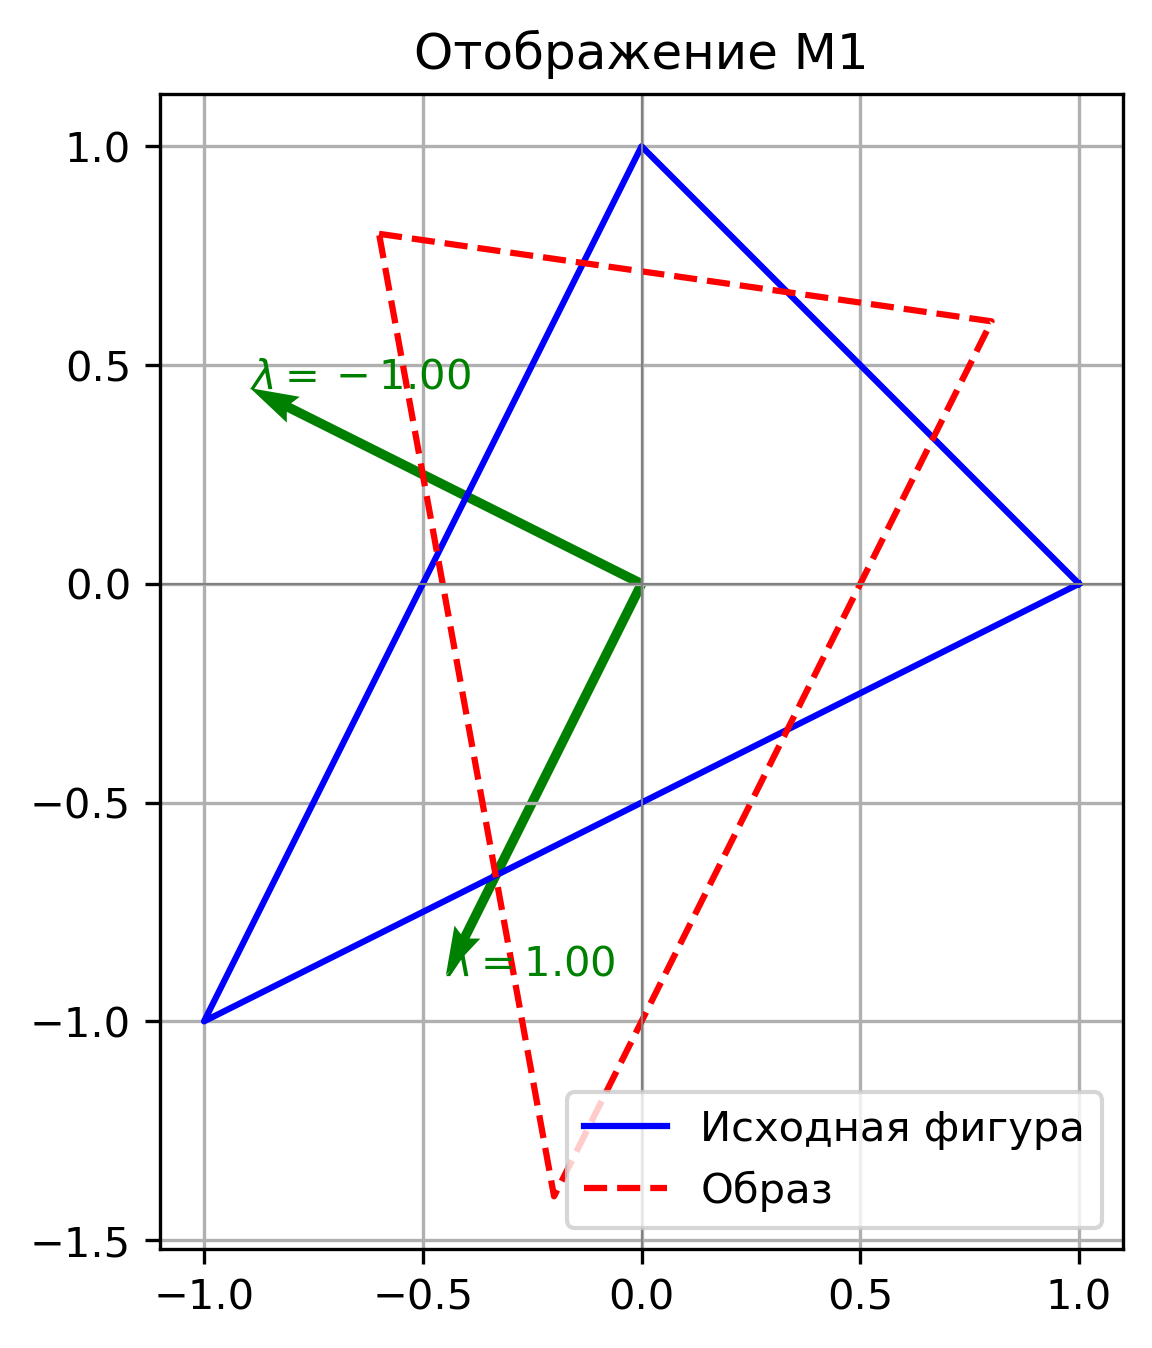
\includegraphics[width=\linewidth]{plots/M1.png}
    \caption{$M_1$}
  \end{subfigure}\hfill
  \begin{subfigure}[b]{0.3\textwidth}
    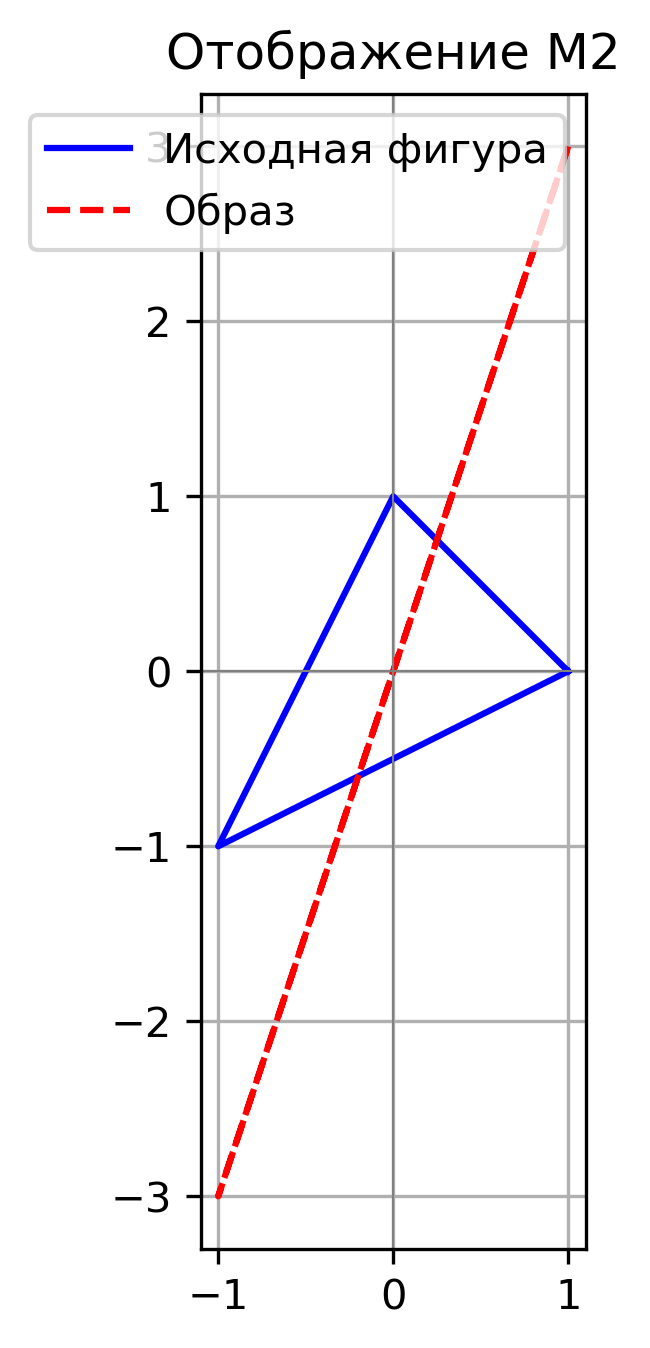
\includegraphics[width=\linewidth]{plots/M2.png}
    \caption{$M_2$}
  \end{subfigure}\hfill
  \begin{subfigure}[b]{0.3\textwidth}
    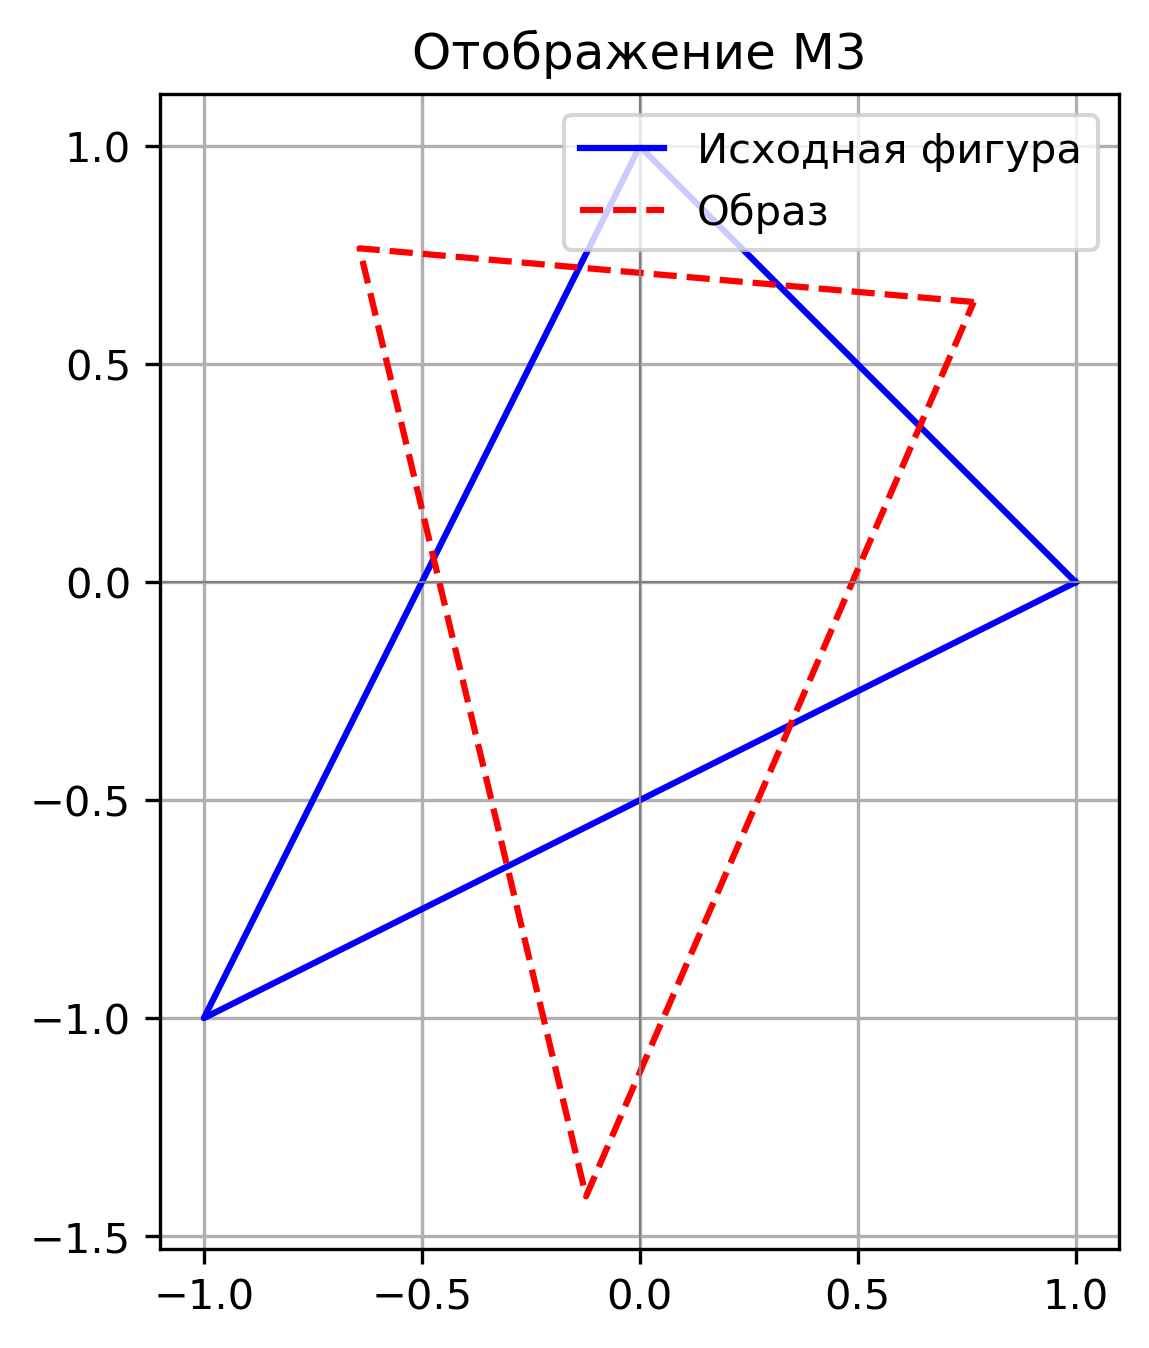
\includegraphics[width=\linewidth]{plots/M3.png}
    \caption{$M_3$}
  \end{subfigure}

  \vspace{0.5cm}

  \begin{subfigure}[b]{0.3\textwidth}
    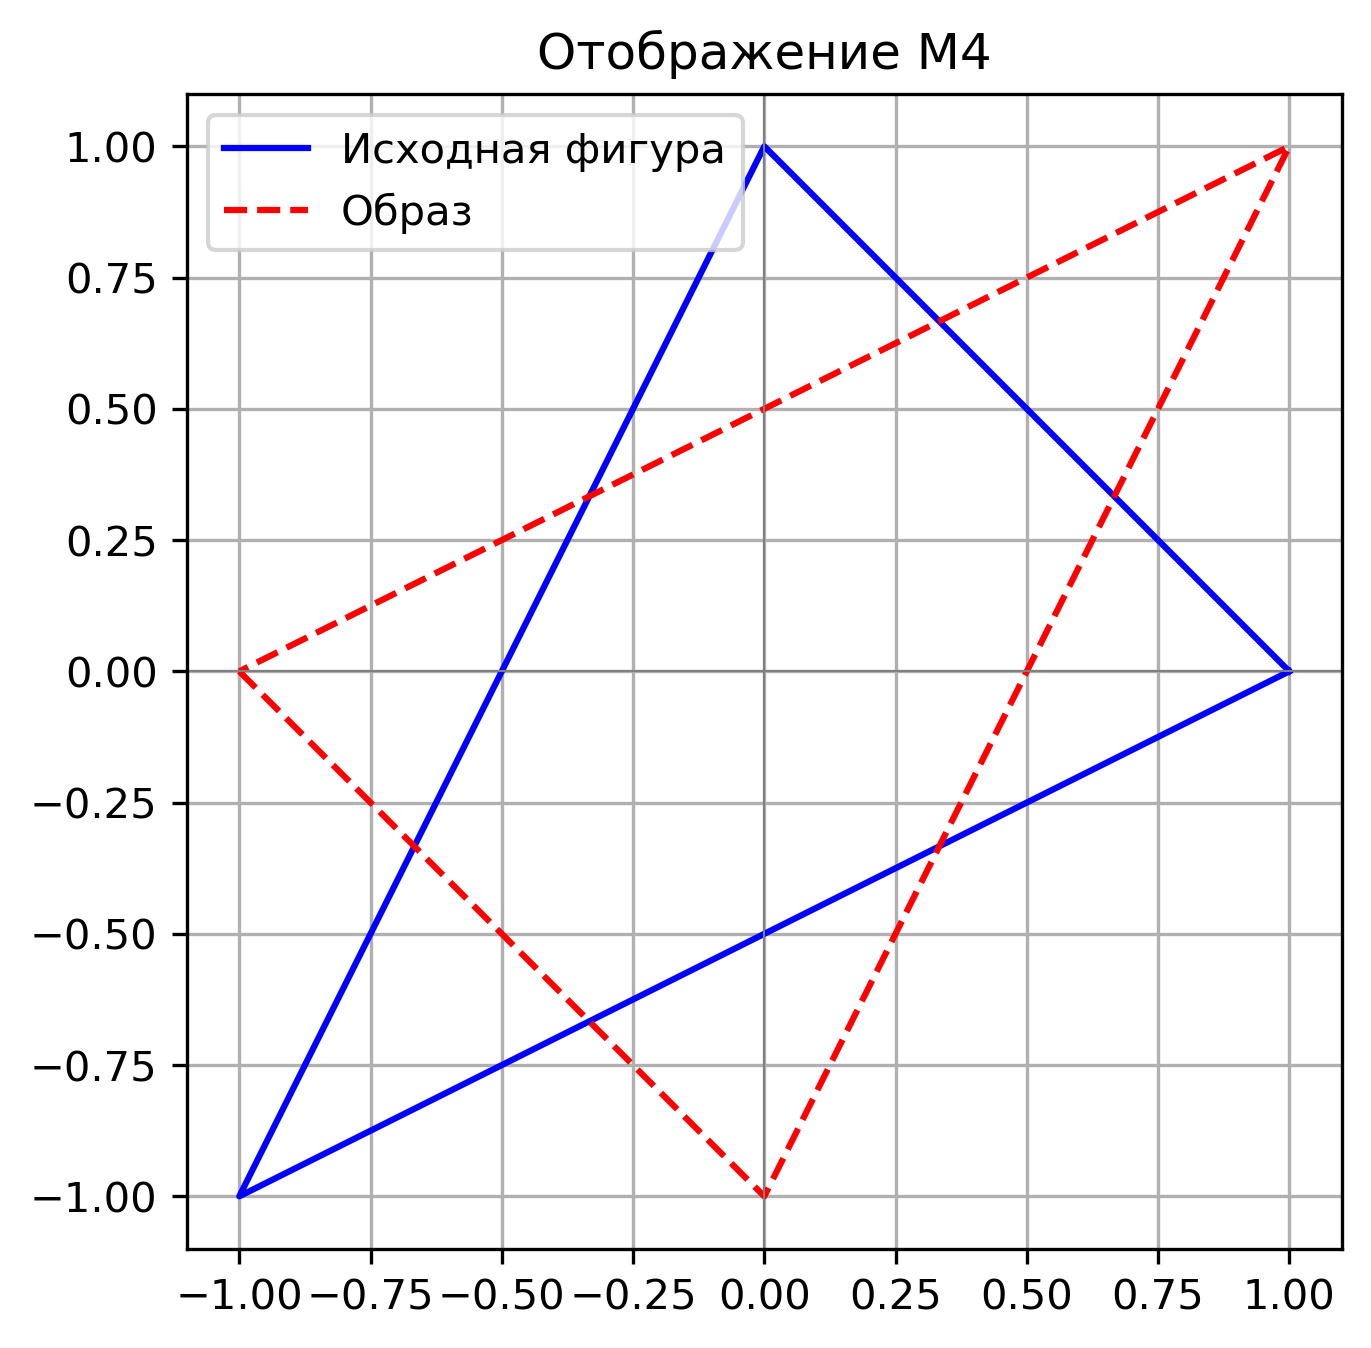
\includegraphics[width=\linewidth]{plots/M4.png}
    \caption{$M_4$}
  \end{subfigure}\hfill
  \begin{subfigure}[b]{0.3\textwidth}
    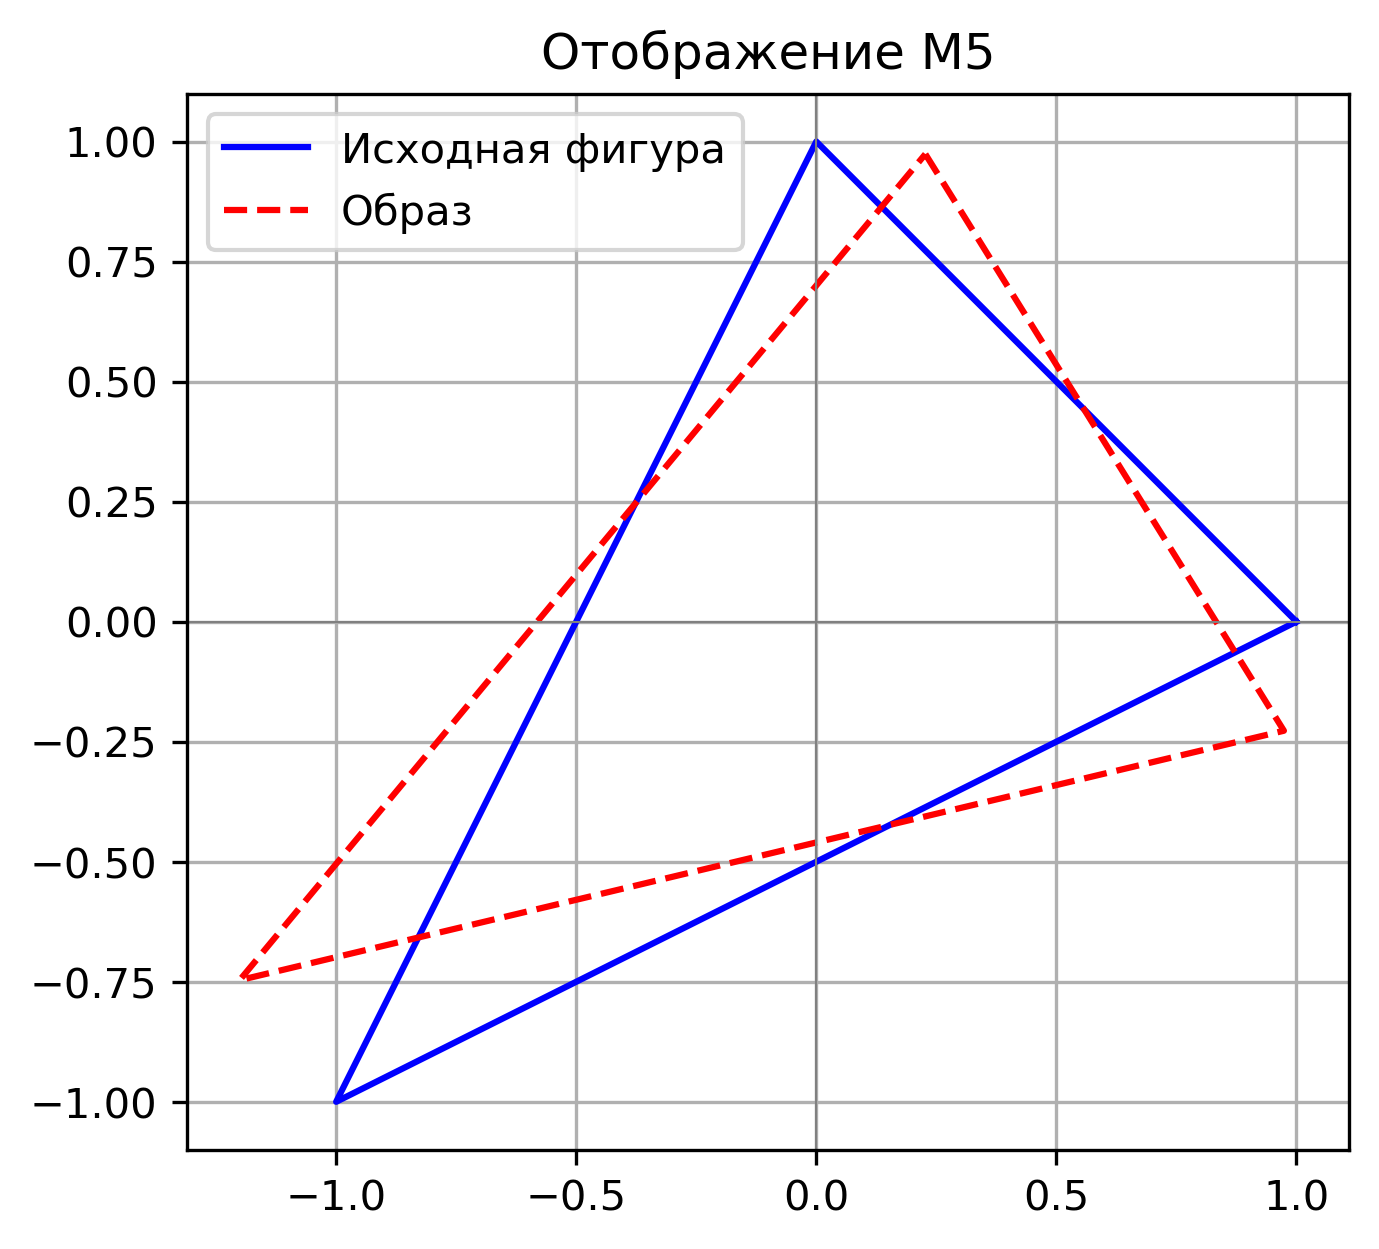
\includegraphics[width=\linewidth]{plots/M5.png}
    \caption{$M_5$}
  \end{subfigure}\hfill
  \begin{subfigure}[b]{0.3\textwidth}
    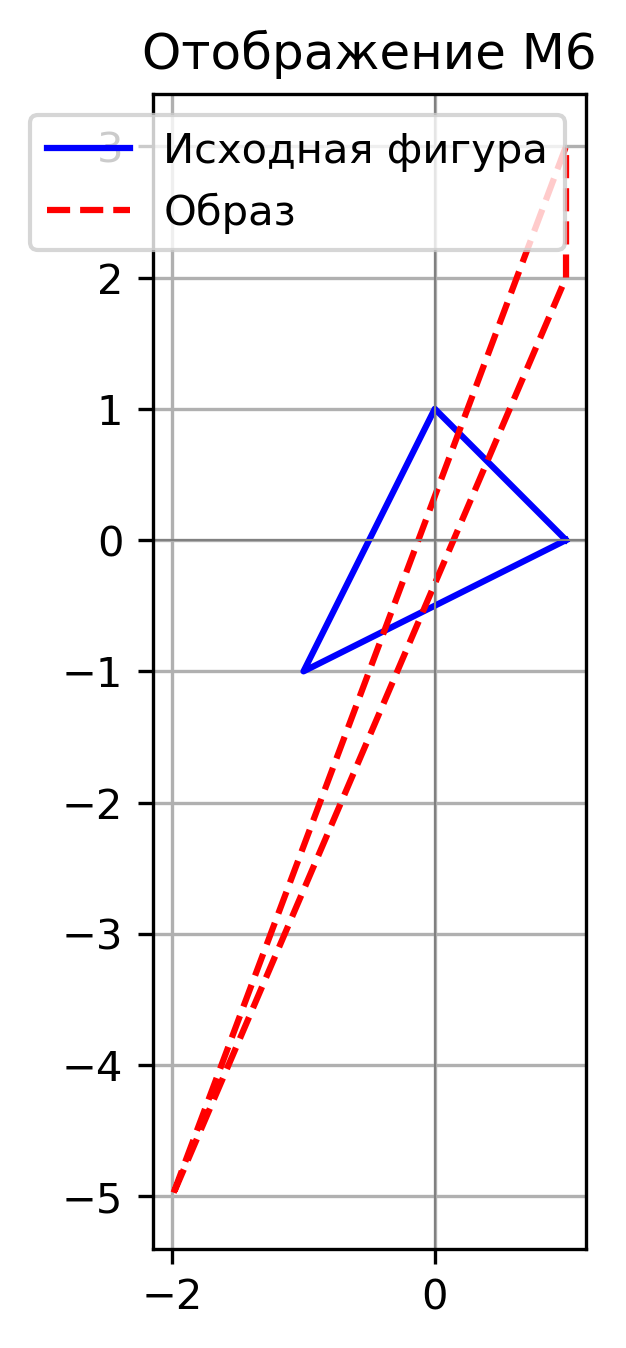
\includegraphics[width=\linewidth]{plots/M6.png}
    \caption{$M_6$}
  \end{subfigure}
  \caption{Отображения $M_1$–$M_6$}
\end{figure}

\clearpage

\begin{figure}[H]
  \centering
  \begin{subfigure}[b]{0.3\textwidth}
    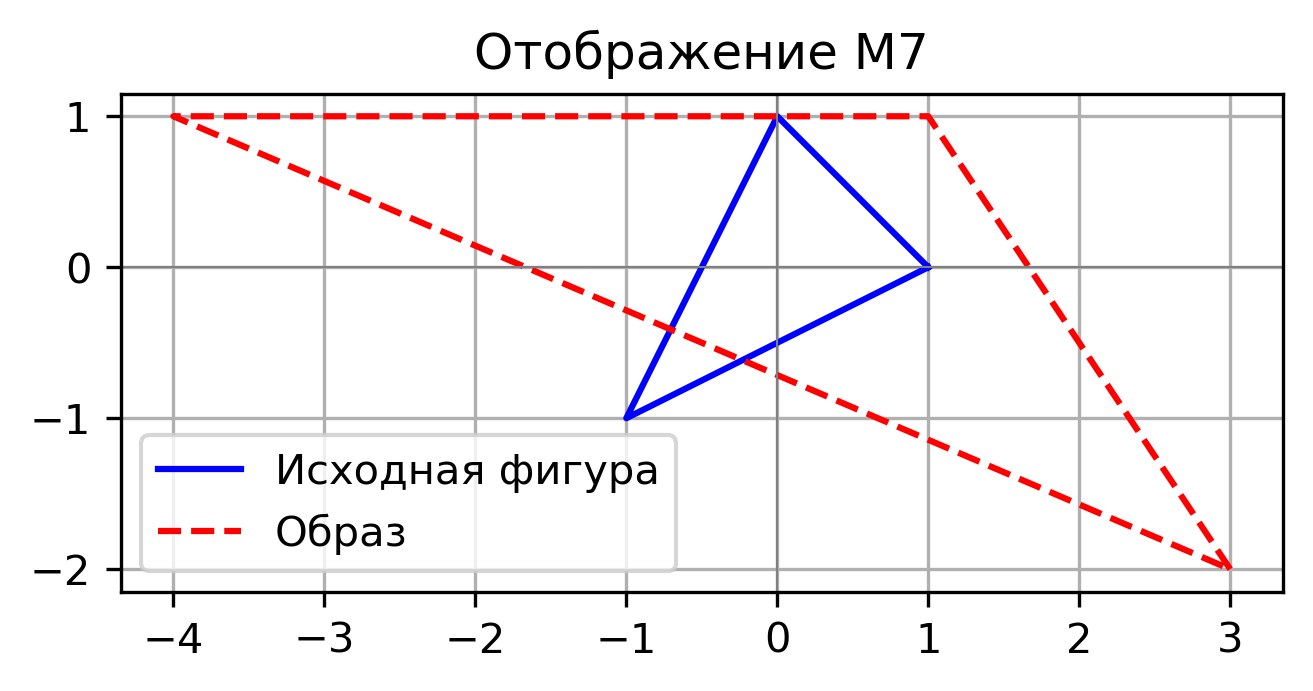
\includegraphics[width=\linewidth]{plots/M7.png}
    \caption{$M_7$}
  \end{subfigure}\hfill
  \begin{subfigure}[b]{0.3\textwidth}
    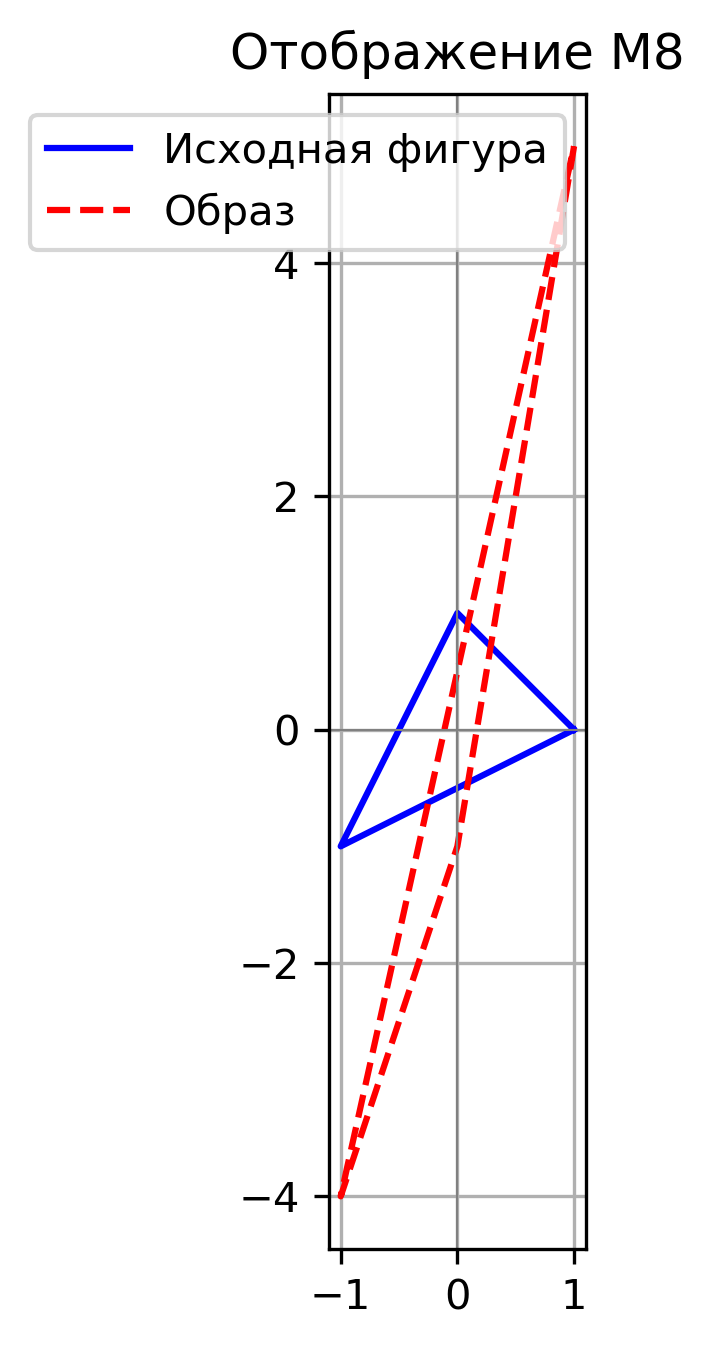
\includegraphics[width=\linewidth]{plots/M8.png}
    \caption{$M_8$}
  \end{subfigure}\hfill
  \begin{subfigure}[b]{0.3\textwidth}
    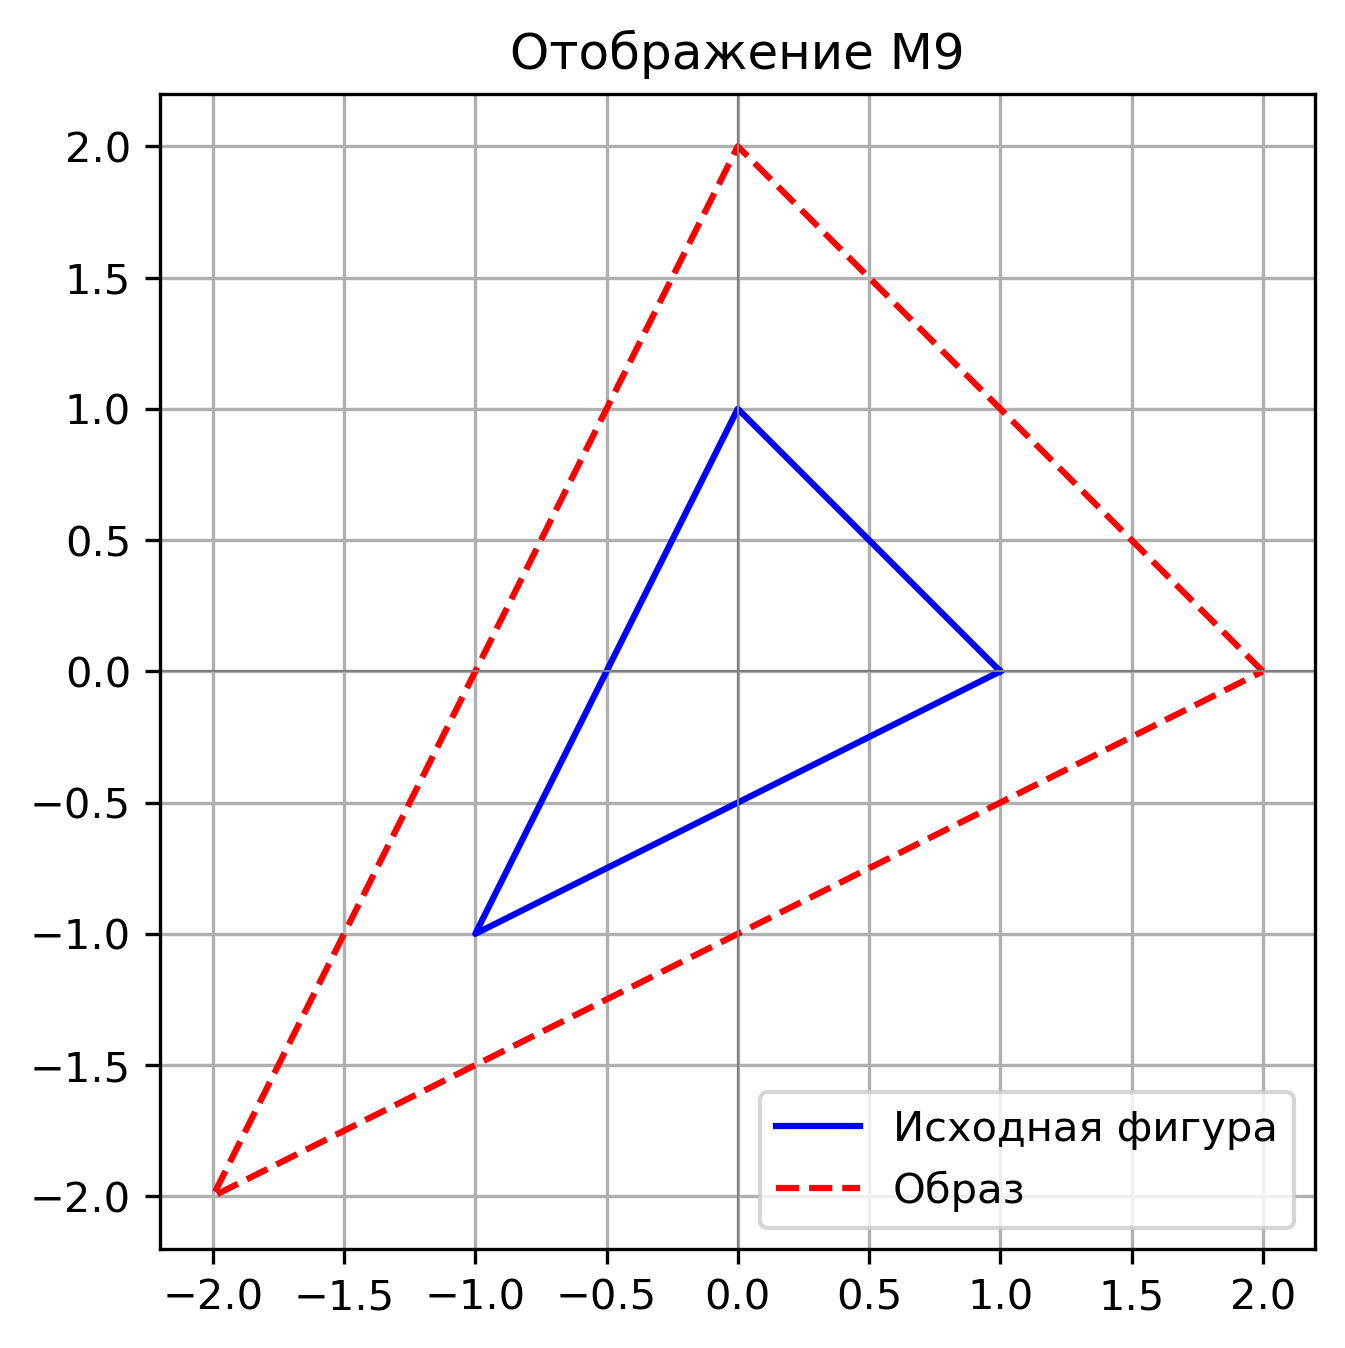
\includegraphics[width=\linewidth]{plots/M9.png}
    \caption{$M_9$}
  \end{subfigure}

  \vspace{0.5cm}

  \begin{subfigure}[b]{0.3\textwidth}
    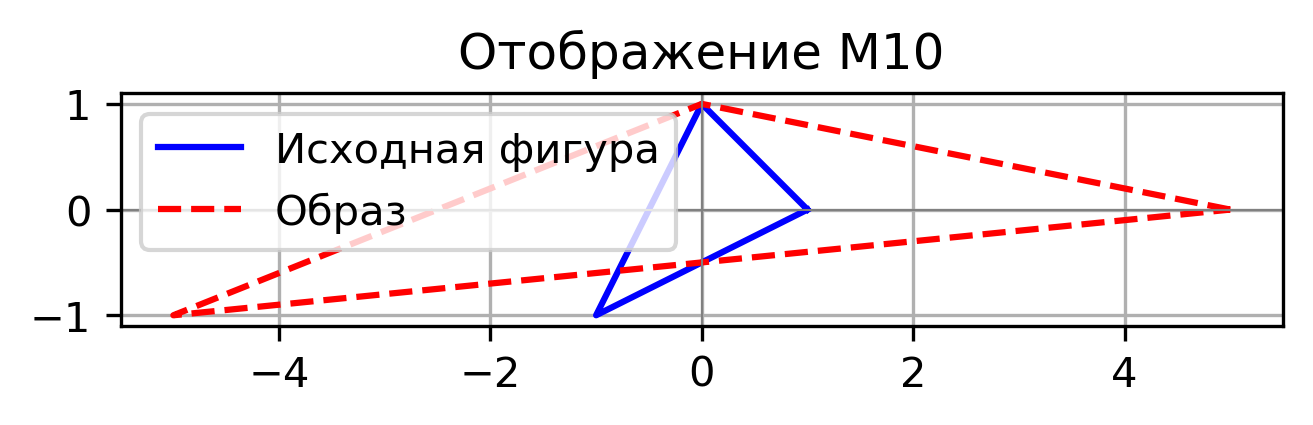
\includegraphics[width=\linewidth]{plots/M10.png}
    \caption{$M_{10}$}
  \end{subfigure}\hfill
  \begin{subfigure}[b]{0.3\textwidth}
    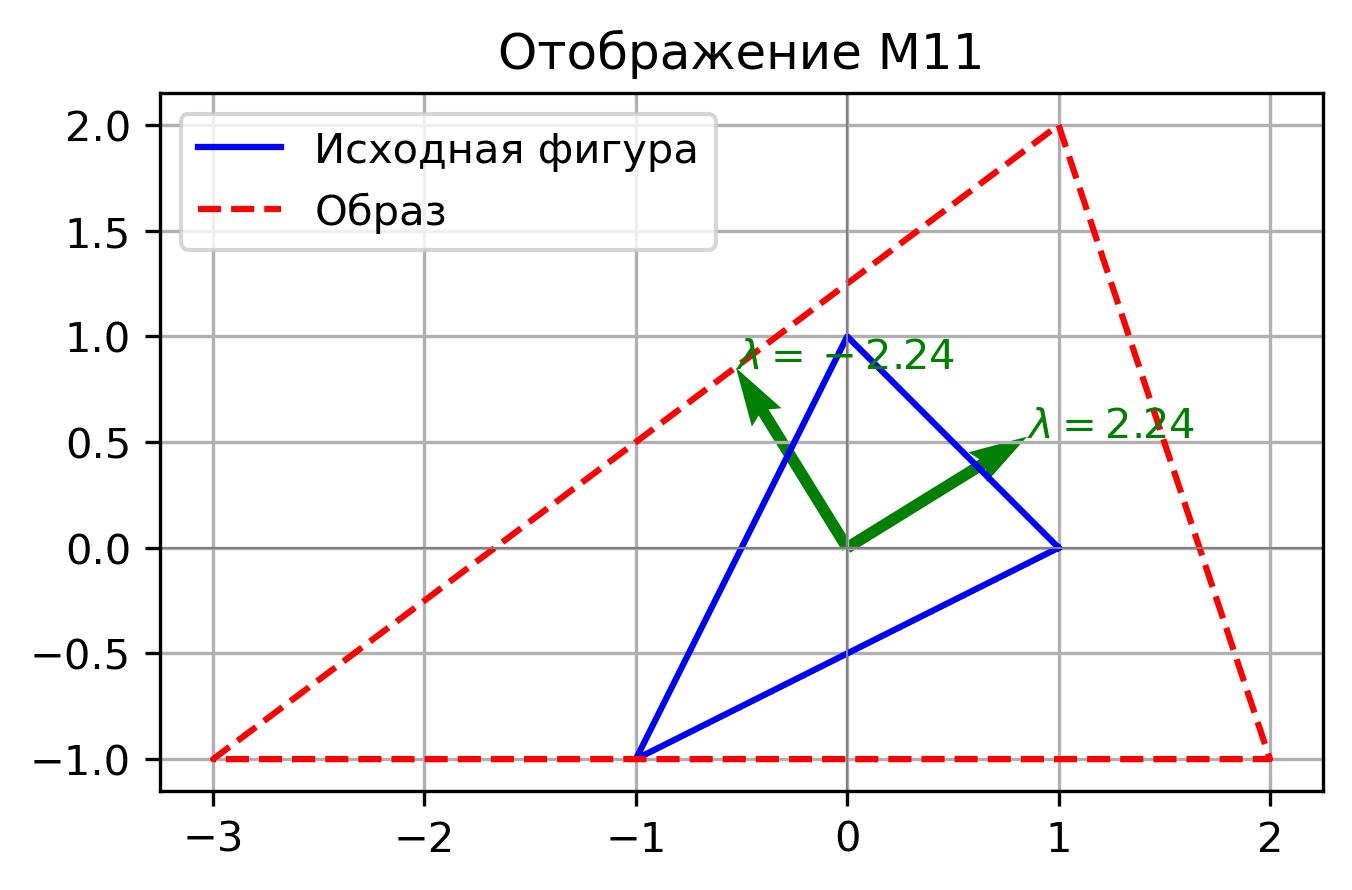
\includegraphics[width=\linewidth]{plots/M11.png}
    \caption{$M_{11}$}
  \end{subfigure}\hfill
  \begin{subfigure}[b]{0.3\textwidth}
    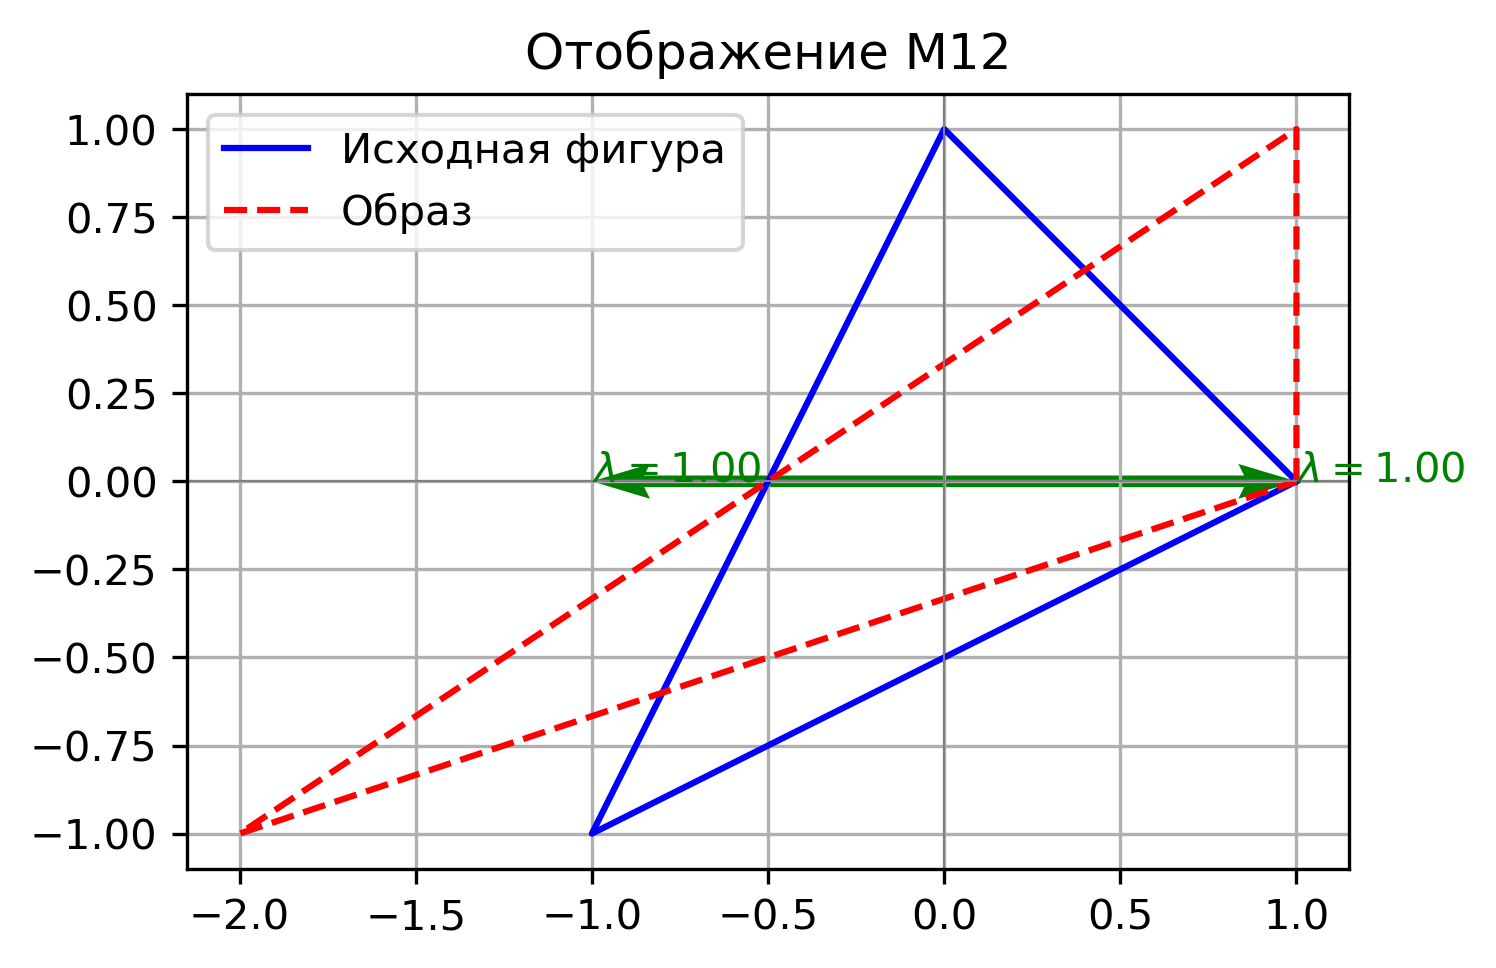
\includegraphics[width=\linewidth]{plots/M12.png}
    \caption{$M_{12}$}
  \end{subfigure}
  \caption{Отображения $M_7$–$M_{12}$}
\end{figure}

\begin{figure}[H]
  \centering
  \begin{subfigure}[b]{0.3\textwidth}
    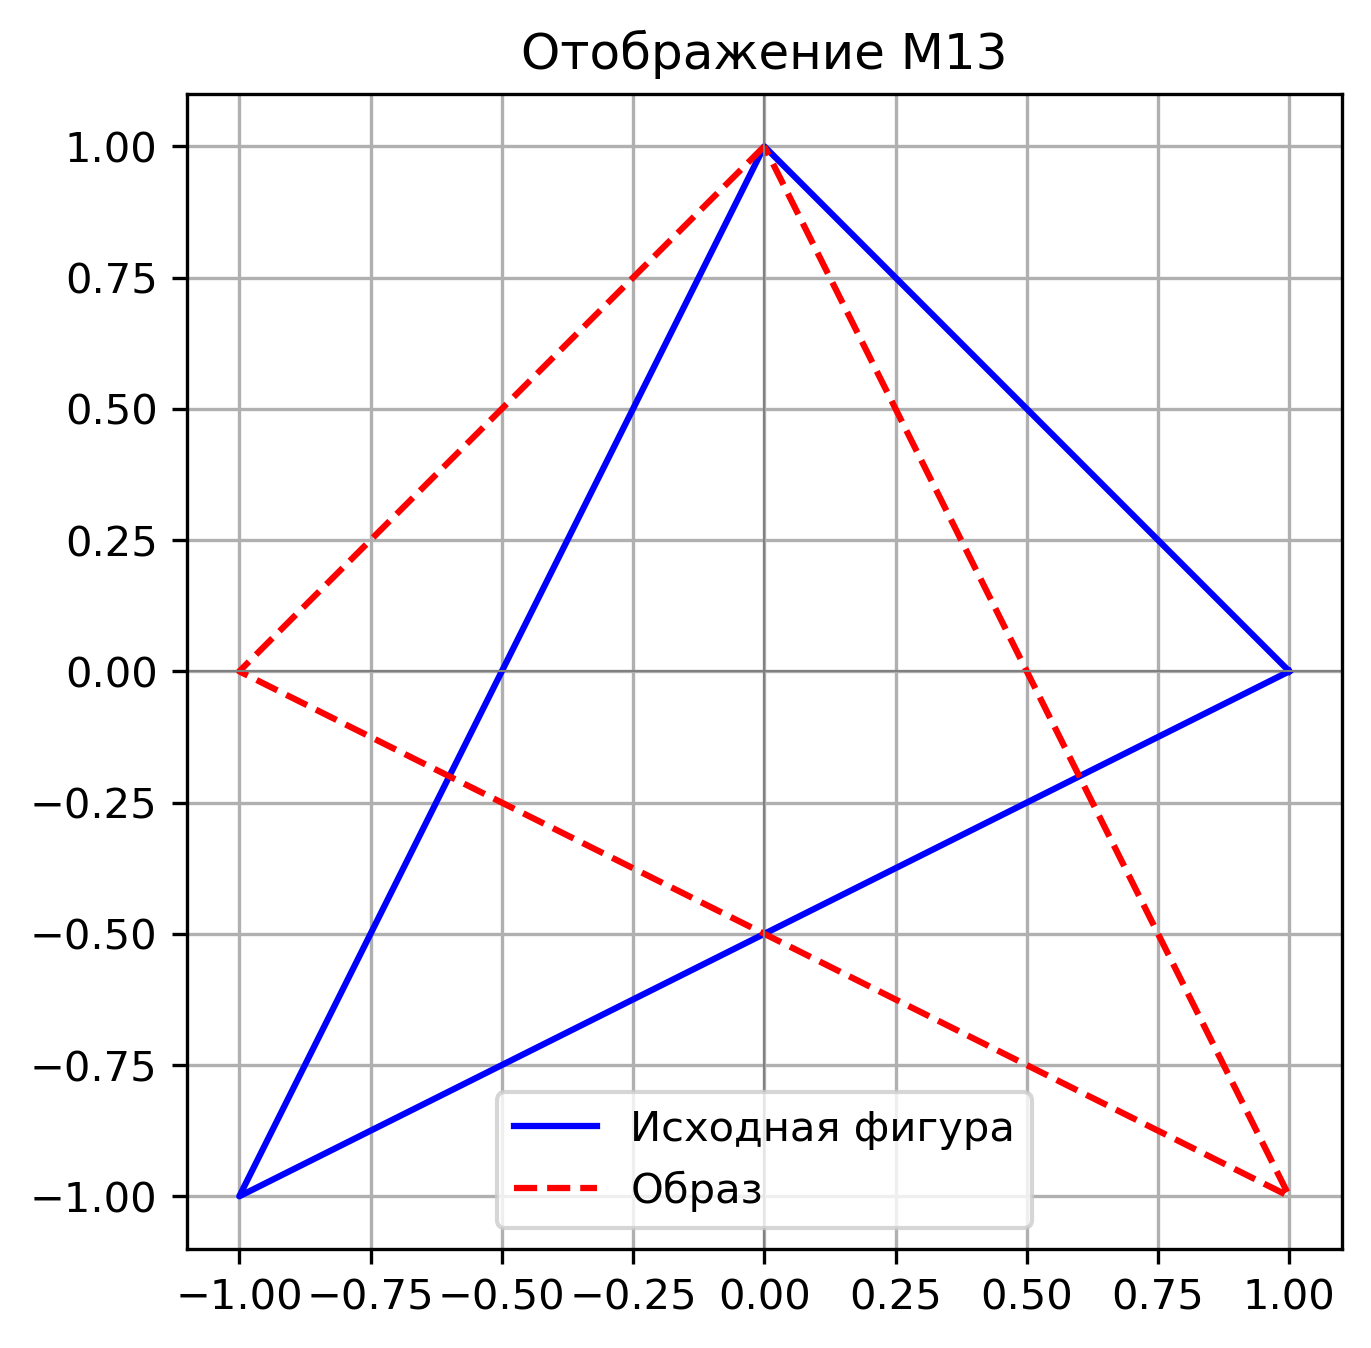
\includegraphics[width=\linewidth]{plots/M13.png}
    \caption{$M_{13}$}
  \end{subfigure}\hfill
  \begin{subfigure}[b]{0.3\textwidth}
    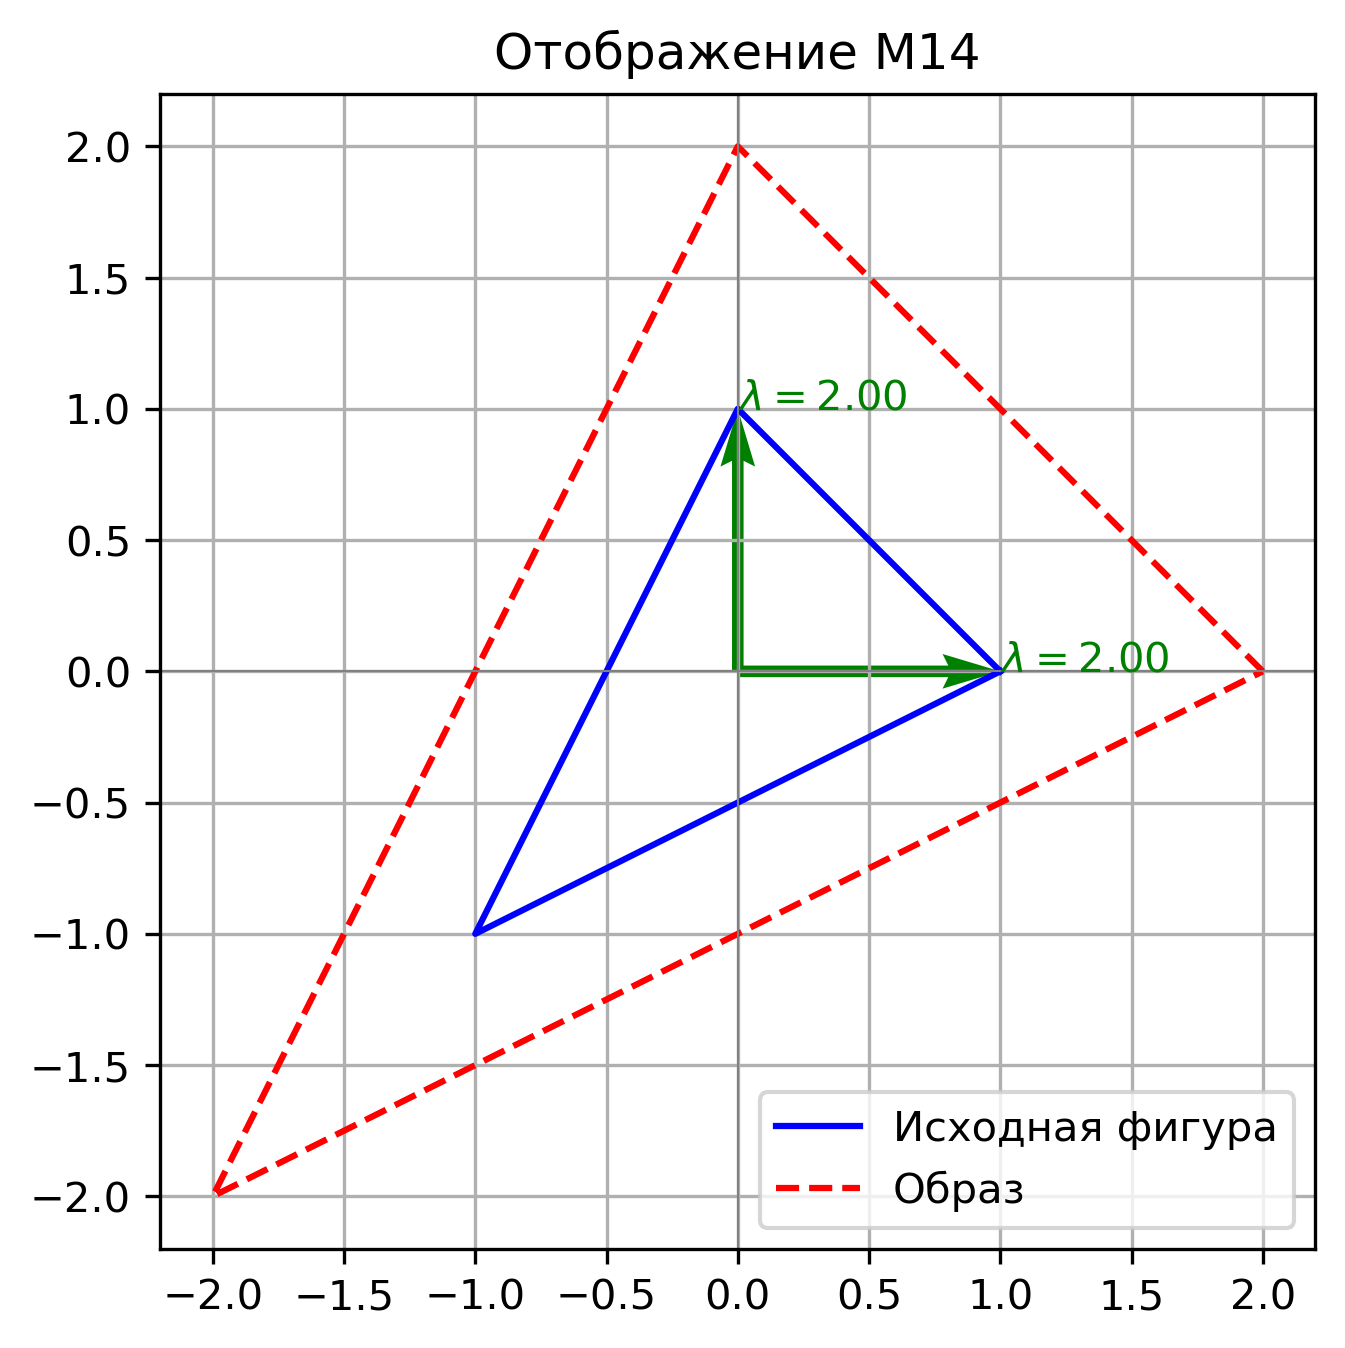
\includegraphics[width=\linewidth]{plots/M14.png}
    \caption{$M_{14}$}
  \end{subfigure}\hfill
  \begin{subfigure}[b]{0.3\textwidth}
    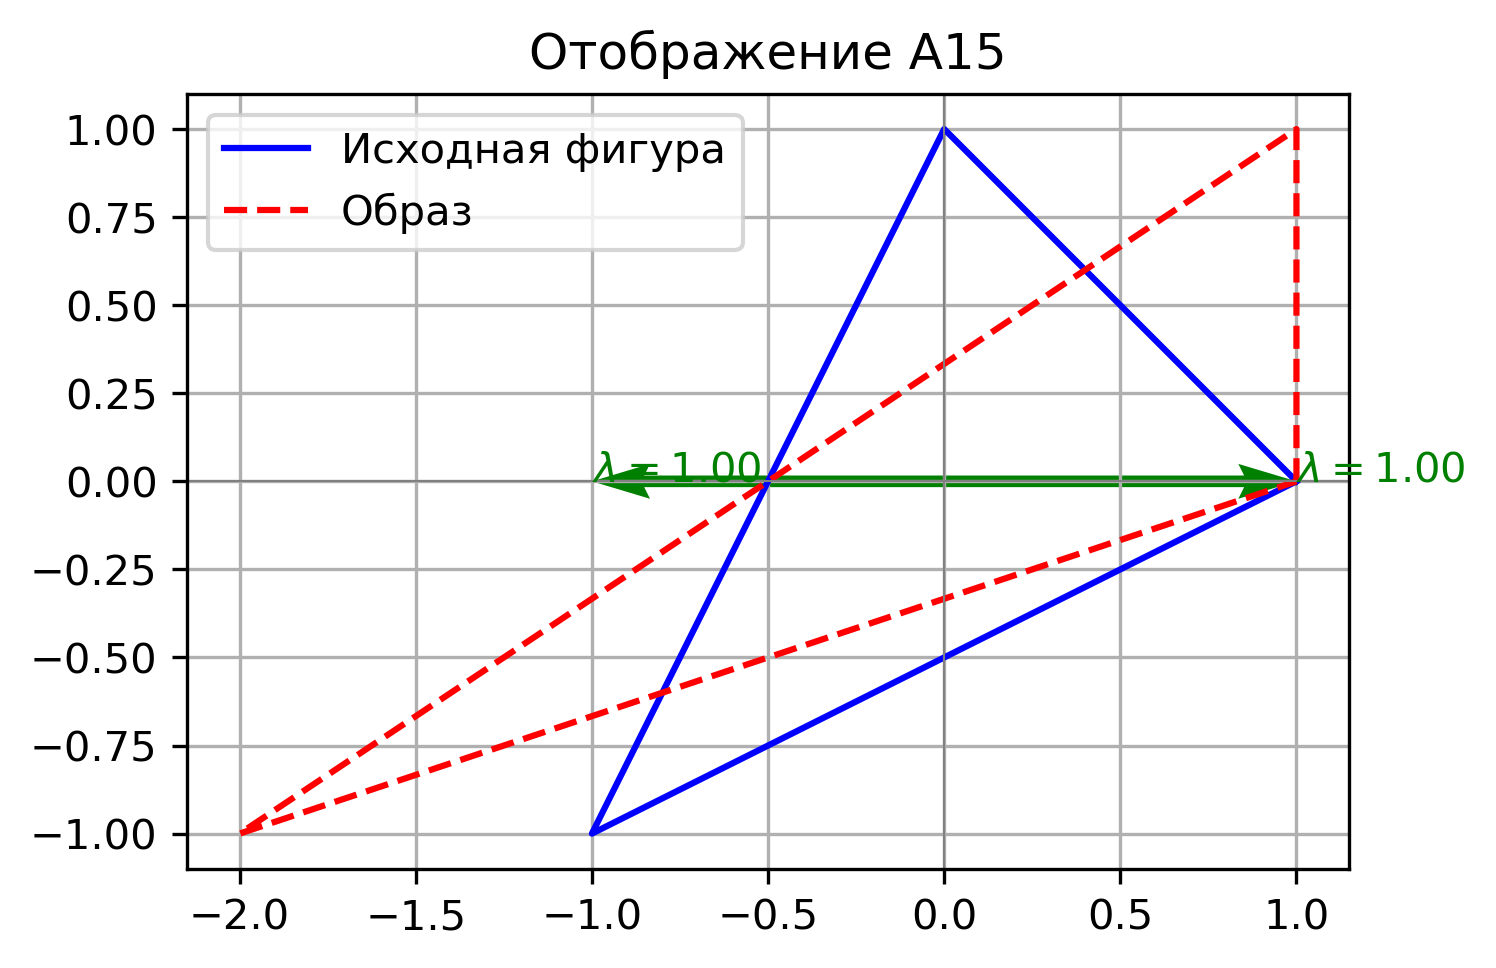
\includegraphics[width=\linewidth]{plots/A15.png}
    \caption{$A_{15}$}
  \end{subfigure}

  \vspace{0.5cm}

  \begin{subfigure}[b]{0.3\textwidth}
    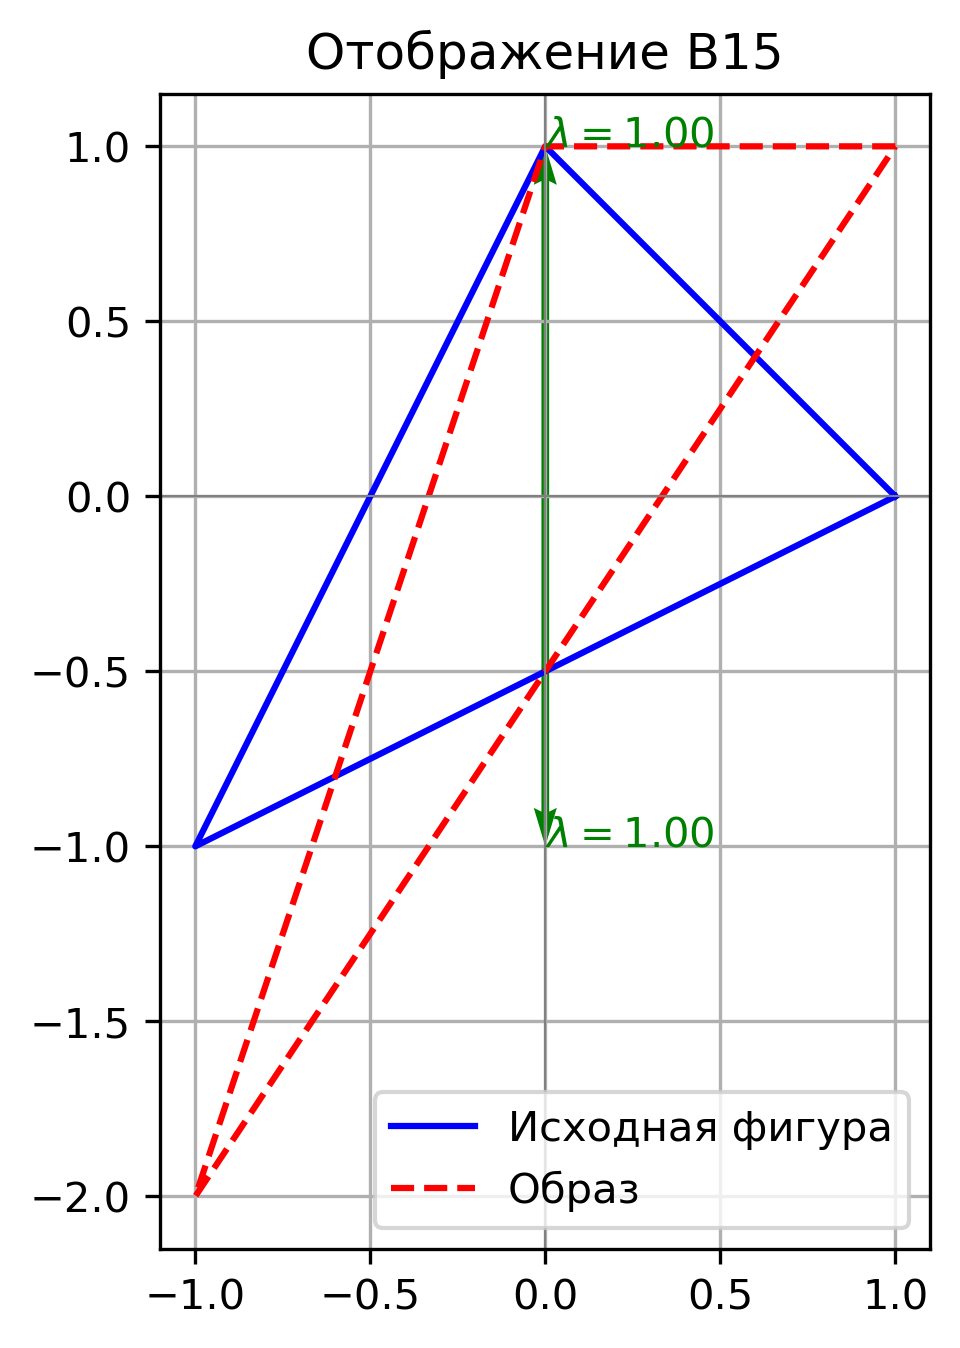
\includegraphics[width=\linewidth]{plots/B15.png}
    \caption{$B_{15}$}
  \end{subfigure}\hfill
  \begin{subfigure}[b]{0.3\textwidth}
    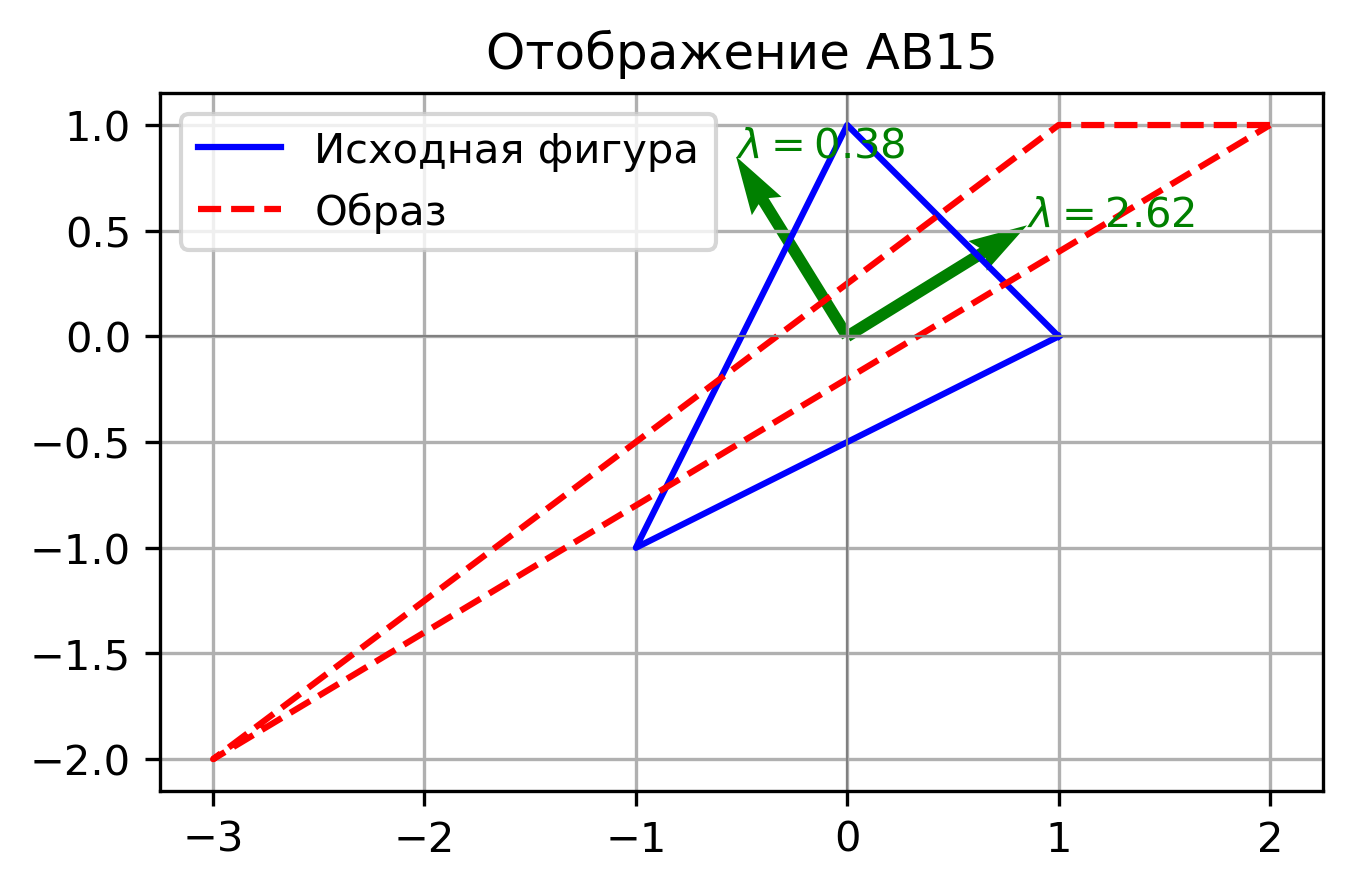
\includegraphics[width=\linewidth]{plots/AB15.png}
    \caption{$A_{15}B_{15}$}
  \end{subfigure}\hfill
  \begin{subfigure}[b]{0.3\textwidth}
    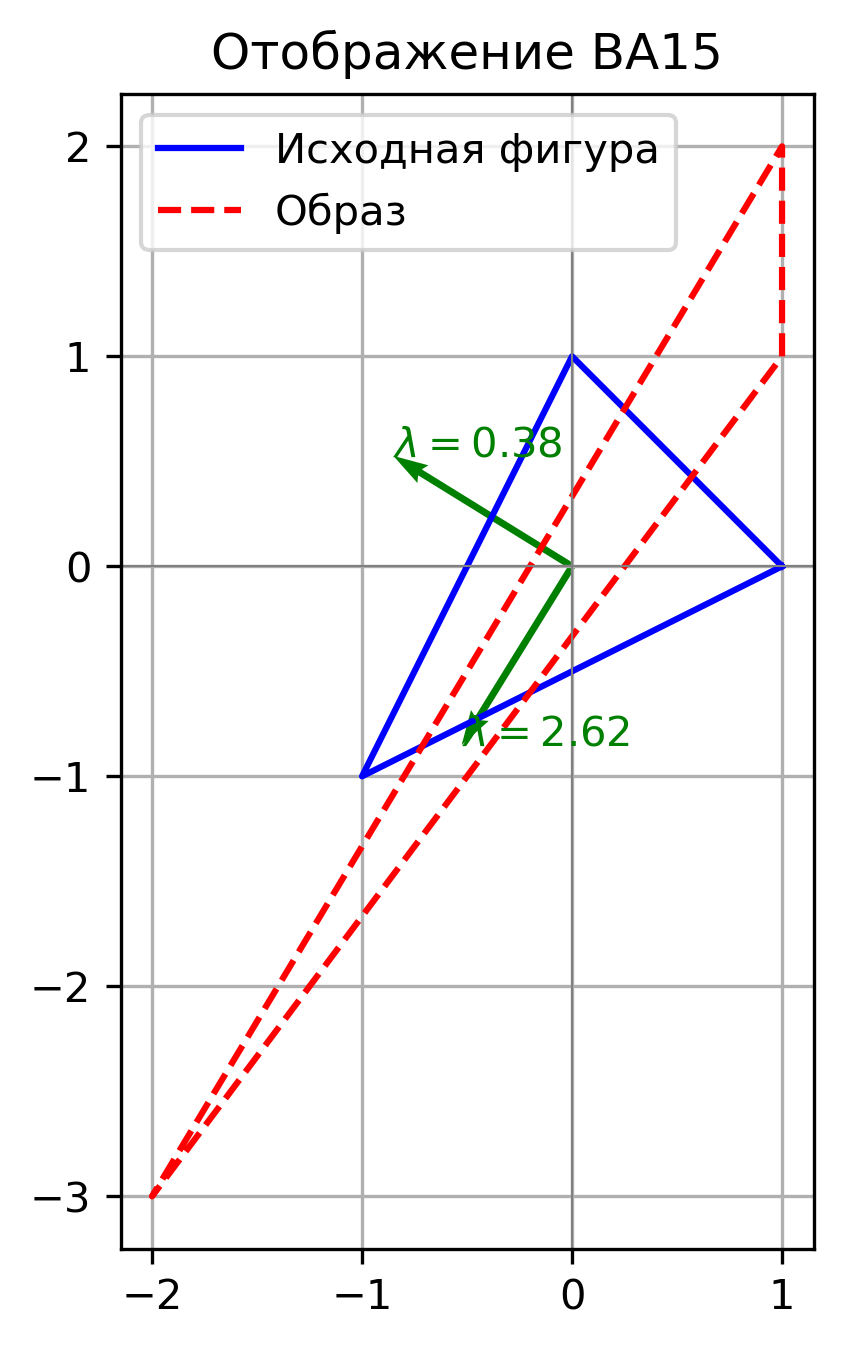
\includegraphics[width=\linewidth]{plots/BA15.png}
    \caption{$B_{15}A_{15}$}
  \end{subfigure}
  \caption{Отображения $M_{13}$–$BA_{15}$}
\end{figure}

\clearpage

\begin{figure}[H]
  \centering
  \begin{subfigure}[b]{0.3\textwidth}
    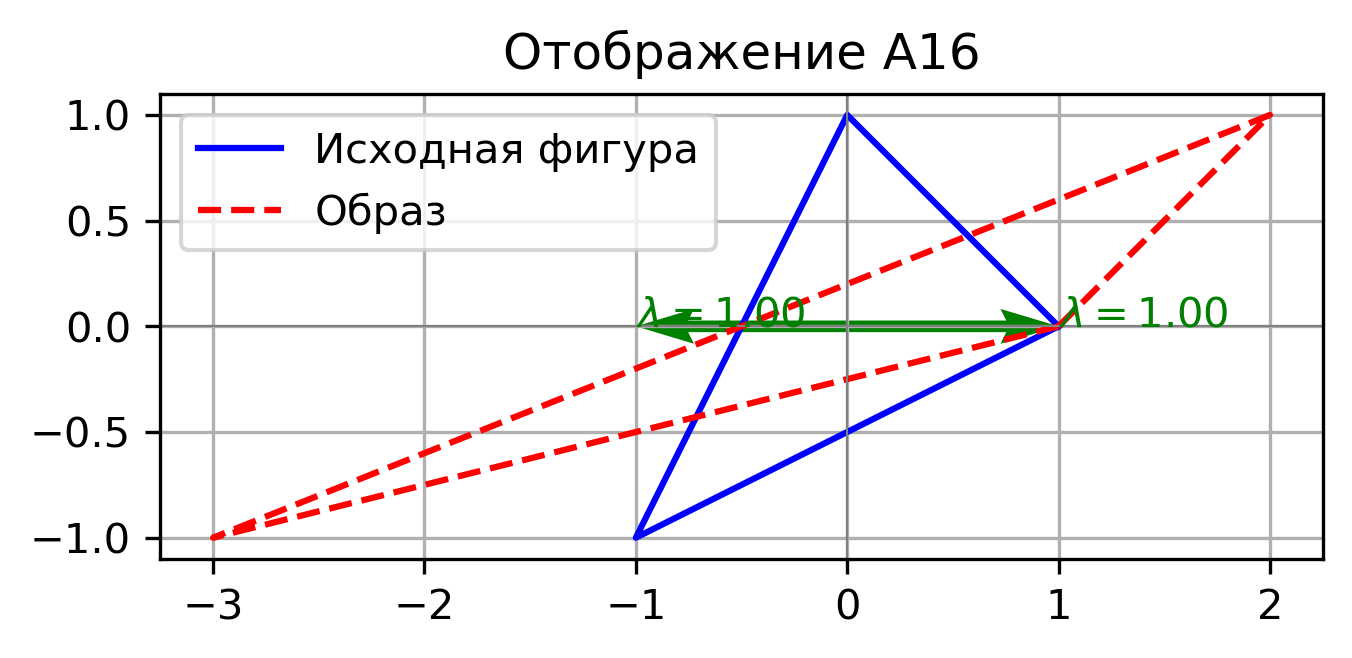
\includegraphics[width=\linewidth]{plots/A16.png}
    \caption{$A_{16}$}
  \end{subfigure}\hfill
  \begin{subfigure}[b]{0.3\textwidth}
    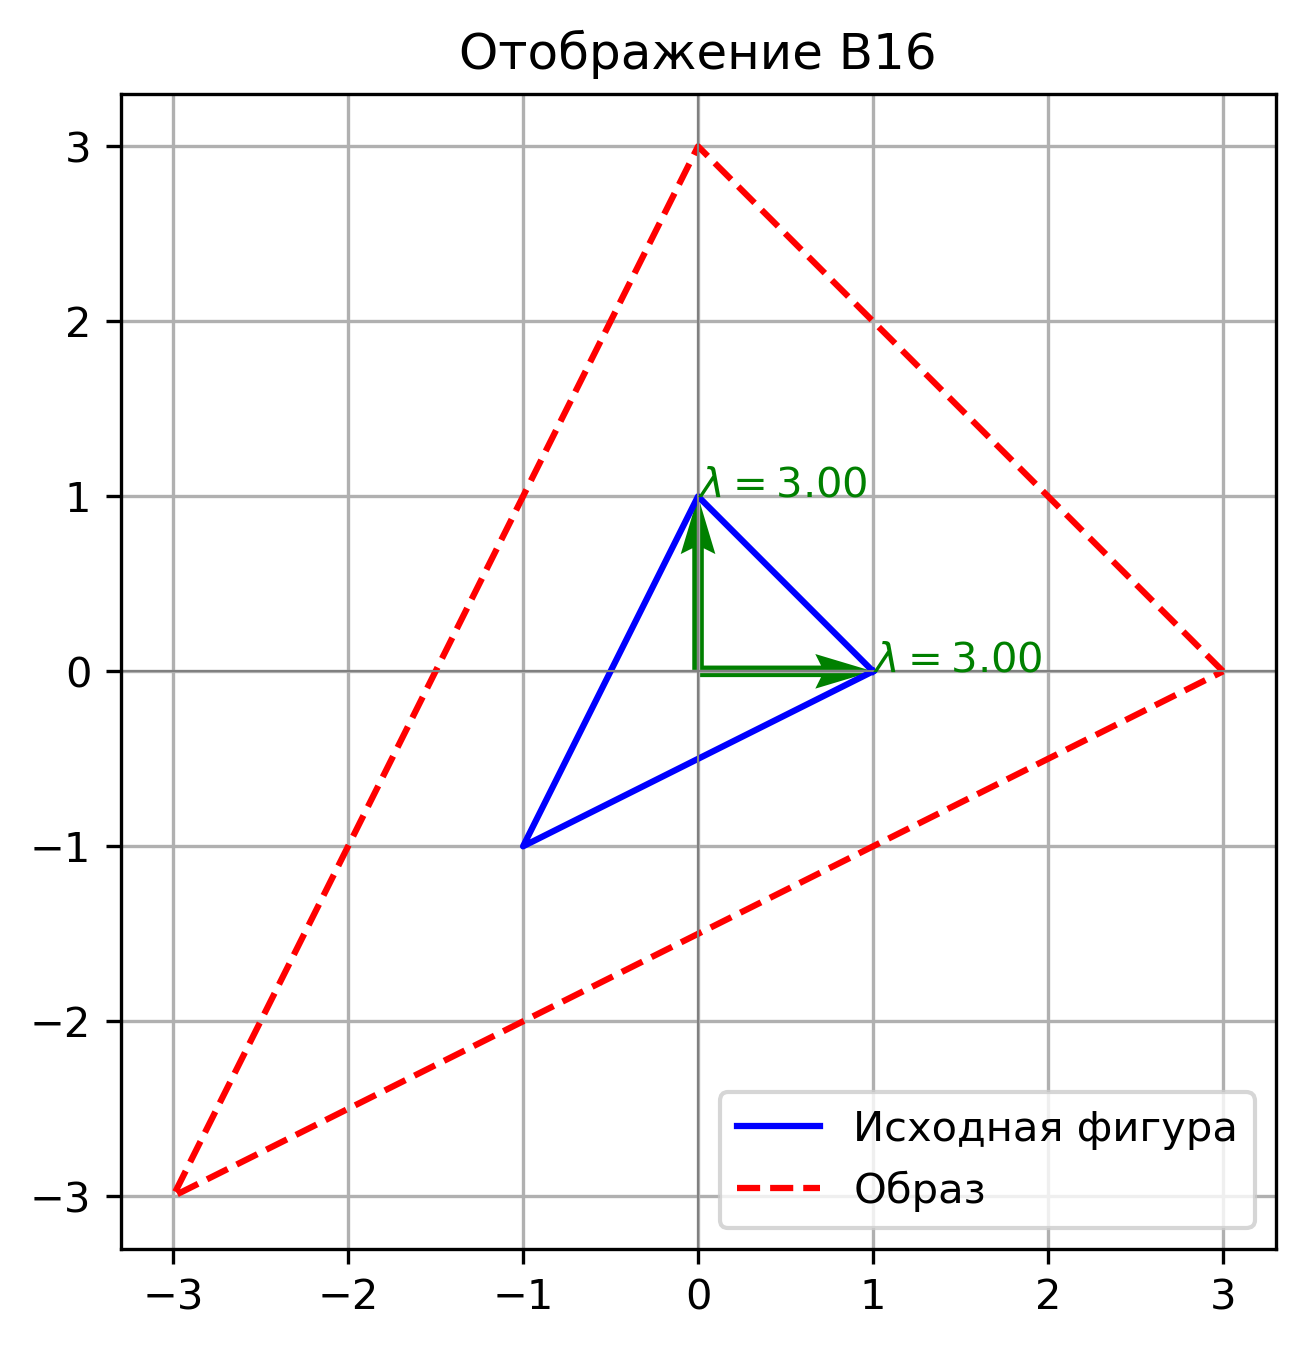
\includegraphics[width=\linewidth]{plots/B16.png}
    \caption{$B_{16}$}
  \end{subfigure}\hfill
  \begin{subfigure}[b]{0.3\textwidth}
    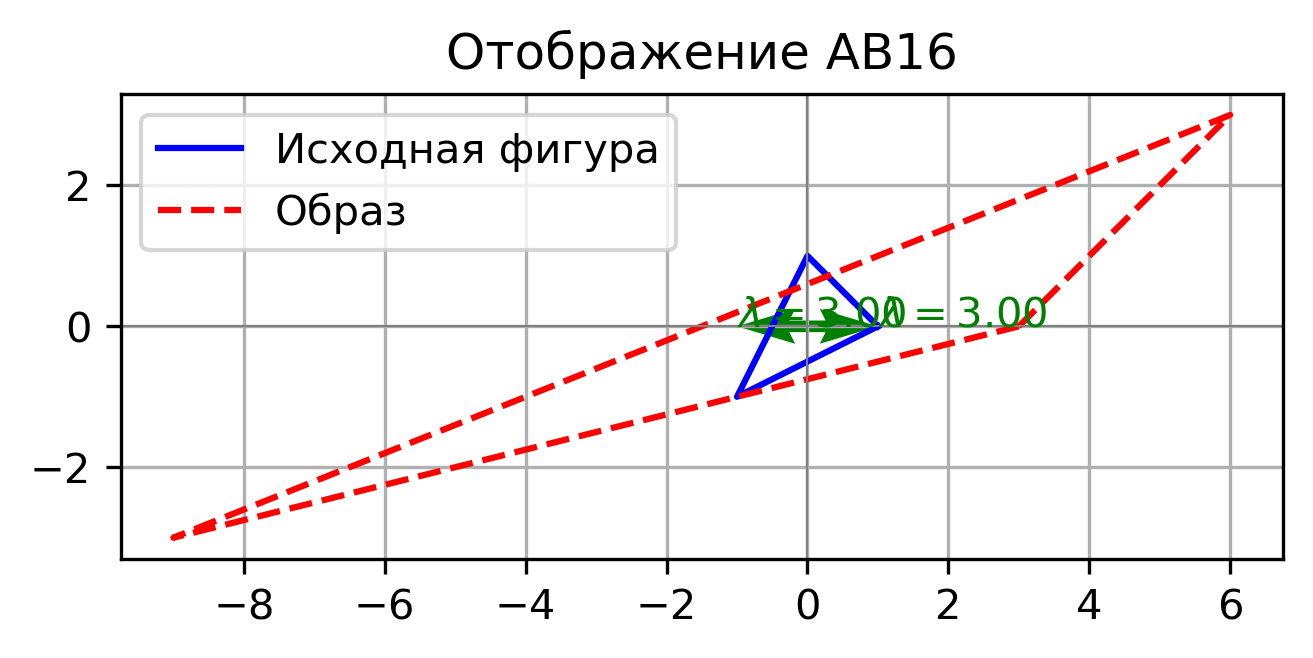
\includegraphics[width=\linewidth]{plots/AB16.png}
    \caption{$A_{16}B_{16}$}
  \end{subfigure}

  \vspace{0.5cm}

  \begin{subfigure}[b]{0.3\textwidth}
    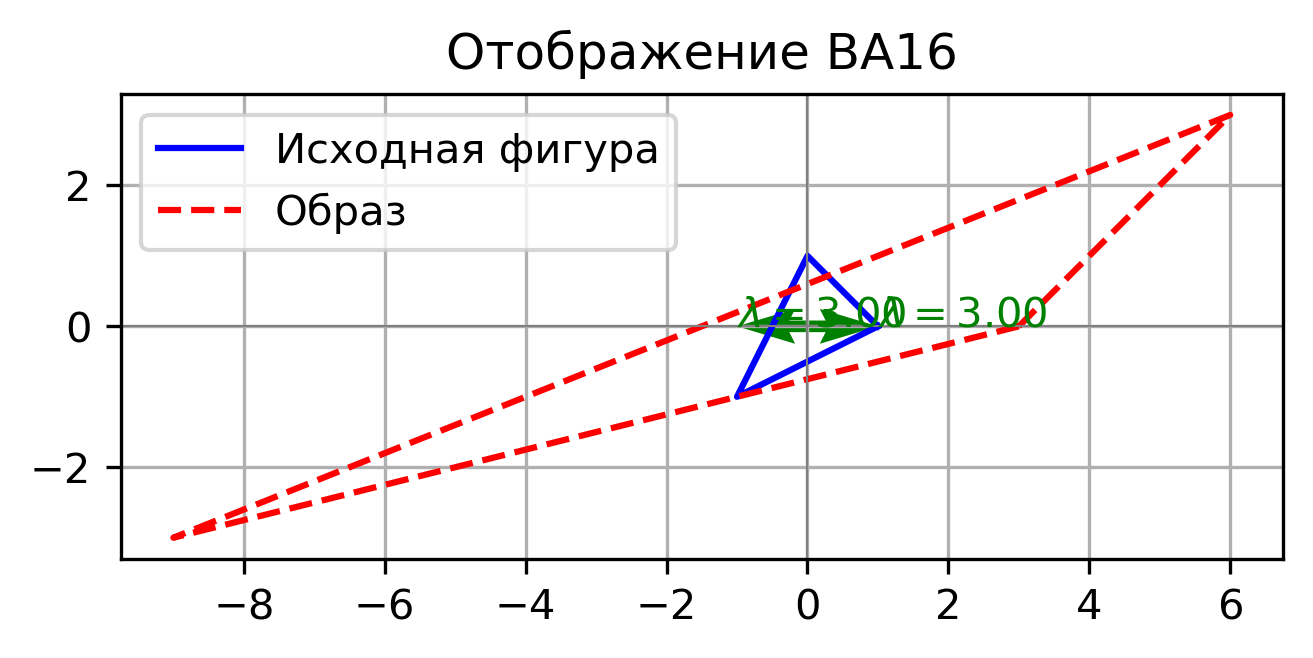
\includegraphics[width=\linewidth]{plots/BA16.png}
    \caption{$B_{16}A_{16}$}
  \end{subfigure}
  \caption{Отображения $A_{16}$–$BA_{16}$}
\end{figure}

\clearpage

% --- Краткие выводы ---
\section*{Выводы}
В работе сконструированы и проанализированы 2D-линейные преобразования, реализующие множество геометрических эффектов: отражения, проекции в прямую, повороты, изотропные и анизотропные масштабирующие отображения, а также примеры некомутации и коммутативности. Для каждого класса даны построения по геометрическим условиям (через образы базисных векторов, ортогональные разложения и жордановы формы), вычислены спектры, образы/ядра и определители. Показано, что симметричность матрицы \emph{обязательна} лишь для отражений через прямую, центральной симметрии, преобразований с ортогональным базисом собственных векторов и скалярных матриц; в остальных случаях она необязательна.                                     % Введение
% \input{3_chap1}                                     % Первая глава
% \input{4_chap2}                                     % Вторая глава
% \input{5_chap3}                                     % Третья глава

\printbibliography[title=Список использованных источников] % Автособираемый список литературы

\end{document}